%Version 3.1 December 2024 -- Springer Nature LaTeX template (sn-jnl)
\documentclass[pdflatex,sn-mathphys-num]{sn-jnl}

\usepackage{graphicx}%
\usepackage{multirow}%
\usepackage{amsmath,amssymb,amsfonts}%
\usepackage{amsthm}%
\usepackage{mathrsfs}%
\usepackage[title]{appendix}%
\usepackage{xcolor}%
\usepackage{textcomp}%
\usepackage{manyfoot}%
\usepackage{booktabs}%
\usepackage{algorithm}%
\usepackage{algorithmicx}%
\usepackage{algpseudocode}%
\usepackage{bm}%
\usepackage{bbm}%
\usepackage{longtable}%
\usepackage{tabularx}%
\usepackage{array}%
\usepackage[section]{placeins}%
\usepackage{rotating}%

%% Placeholder for numbers that will be filled from logged experiment results only.
\newcommand{\RES}[1]{\textcolor{red}{[#1]}}
%% Comparison-table symbols.
\newcommand{\yes}{$\checkmark$}
\newcommand{\no}{$\times$}
\newcommand{\na}{--}
%% Column type for tabularx with centred content.
\newcolumntype{Y}{>{\centering\arraybackslash}X}
%% Shorthands.
\newcommand{\Lann}{\mathcal{L}_{\mathrm{ann}}}


%% Theorem-like environments (styles defined by sn-jnl.cls).
\theoremstyle{thmstyleone}%
\newtheorem{proposition}{Proposition}%
\theoremstyle{thmstyletwo}%
\newtheorem{remark}{Remark}%

\raggedbottom

\begin{document}

\title[Hybrid text-anchored learning from heterogeneously annotated ECG databases]{Hybrid text-anchored learning from heterogeneously annotated ECG databases for cross-database and open-vocabulary 12-lead ECG diagnosis}

\author*[1]{\fnm{Md. Samiul} \sur{Alom}}\email{samiulalom090@gmail.com}

\author[2]{\fnm{Rukaiya} \sur{Taha}}\email{taharukaiyah@gmail.com}

\affil*[1]{\orgdiv{Miyan Research Institute}, \orgname{International University of Business Agriculture and Technology (IUBAT)}, \orgaddress{\city{Dhaka}, \country{Bangladesh}}}

\affil[2]{\orgdiv{Department of Computer Science and Engineering}, \orgname{International University of Business Agriculture and Technology (IUBAT)}, \orgaddress{\city{Dhaka}, \country{Bangladesh}}}



\abstract{\textbf{Purpose:} Public 12-lead electrocardiogram (ECG) databases each annotate a different subset of diagnoses, so pooling them for scale silently turns ``never coded here'' into ``absent'' and rewards models for recognizing the source database. We study whether a model can learn only from the labels each source observes, transfer to a database that contributed no training data, and score diagnoses for which no training label exists. \textbf{Methods:} We propose a hybrid classifier in which a one-dimensional squeeze-and-excitation residual encoder is read by two heads: a linear head with one weight vector per diagnosis, and a text-anchored label-query head in which frozen embeddings of short guideline-based diagnosis descriptions cross-attend to the ECG tokens and are scored by cosine similarity, so that it has no diagnosis-specific weights. Diagnoses annotated in training are scored by the mean of both heads, unannotated diagnoses by the text head alone. Both heads are trained with an asymmetric loss restricted to source-annotated entries, with clinical implication completion and weight averaging. We evaluate leave-one-database-out over four public databases from three countries (87{,}661 recordings, 43 diagnoses), separating diagnoses seen in training from those annotated only in the held-out database, and in a controlled annotation-removal experiment on PTB-XL, against seven label-handling and domain-generalization baselines trained under identical conditions, with three seeds each. \textbf{Results:} On seen diagnoses the method obtained the highest mean macro AUROC (86.6) and AUPRC (33.0); it was significantly better than six of the seven baselines across folds and seeds (Holm-adjusted Wilcoxon $p\le0.014$) and level with the masked-loss baseline ($+0.25$ points, $p=0.052$). Masking unannotated entries improved on naive pooling by 0.7 points, whereas no domain-generalization method improved on masking. On five diagnoses that no training database annotated, the method reached a macro AUROC of 67.0 where all baselines were at chance (51--53) and a report-pretrained ECG--language model (MERL) reached 48.0--62.6. Over 120 systematically withheld diagnosis--database pairs, zero-shot scoring from the description alone reached 70.2 (88\% of pairs above chance), against 77.3 for MERL, which was better on frequent rhythm diagnoses and worse on several morphology findings. \textbf{Conclusion:} Correct handling of missing annotation matters more for cross-database ECG transfer than domain-generalization penalties, and a hybrid text-anchored head adds the ability to score unlabeled diagnoses from a description without loss of accuracy on labeled ones, complementing report-pretrained models.}

\keywords{Electrocardiogram, Multi-source learning, Partial labels, Domain generalization, Text-anchored label embeddings, Open-vocabulary diagnosis}

\maketitle

%=====================================================================
\section{Introduction}\label{sec:intro}
%=====================================================================

Cardiovascular diseases (CVDs) are the leading cause of death worldwide: the number of prevalent cases nearly doubled from 271 million in 1990 to 523 million in 2019, and CVD deaths rose from 12.1 million to 18.6 million over the same period~\cite{roth2020gbd}. The 12-lead electrocardiogram (ECG) is the most widely used cardiac test in this population, and deep neural networks now match or exceed non-specialist physicians on many ECG interpretation tasks~\cite{hannun2019,ribeiro2020,siontis2021}. Most published models, however, are trained and tested on a single database. Their reported accuracy is therefore an in-distribution estimate that says little about how the model behaves in a hospital whose patients, recording hardware, filtering and annotation habits differ from those seen in training. On the widely used PTB-XL benchmark~\cite{wagner2020,strodthoff2021}, for example, architectural refinements now differ by fractions of a point in macro area under the receiver operating characteristic curve (AUROC)~\cite{sharan2025,zhou_leadgraph2026}, whereas the much larger performance drop that occurs when a model is moved to another hospital~\cite{reyna2022,ballas2022} receives far less methodological attention.

A natural remedy is to train on several public databases at once. The PhysioNet/Computing in Cardiology (CinC) Challenges of 2020 and 2021 made this practical by releasing tens of thousands of 12-lead recordings from hospitals in China, Germany, Russia and the United States, all coded with SNOMED-CT diagnoses~\cite{perez2020,reyna2022}; PTB-XL alone contributes 21{,}837 records from 18{,}885 patients~\cite{wagner2020}. Pooling these sources exposes a problem that is easy to overlook: \emph{each database annotates a different subset of diagnoses}. The CPSC2018 database~\cite{liu_cpsc2018}, for instance, was labeled for nine rhythm, conduction and ST-segment classes, whereas other databases code findings such as T-wave abnormalities, axis deviation or low QRS voltage that CPSC2018 never mentions. In the four databases studied here, only 18 of the 43 diagnoses in our vocabulary are annotated by all four databases, 27.9\% of the positive labels in the pooled data belong to diagnoses that at least one database never codes, and 16.7\% of all record--diagnosis entries are unknown rather than negative (Fig.~\ref{fig:annot}). When databases are concatenated, a diagnosis that a hospital never codes is silently interpreted as a confirmed negative. The model is thereby trained to deny findings that may well be present, and the error is systematic: it is correlated with the source, and therefore with the very acquisition characteristics that a cross-hospital model needs to ignore. The organizers of the 2021 Challenge identified heterogeneous labels and populations as a central open issue~\cite{reyna2022}.

Four lines of work address parts of this problem, and each stops short of the setting we study. First, the architectural line builds ever stronger classifiers evaluated in-distribution~\cite{zhao2020cinc,nejedly2021,sharan2025,zhou_leadgraph2026,sethi2025proto}; it assumes a complete label matrix and does not test transfer to a database that contributed no training data. Second, partial-label methods treat unannotated entries as unknown rather than negative~\cite{durand2019,benbaruch2022}; for ECG, Li et al.~\cite{li2024} recovered missing super-classes with a category mapping and masked predictions for dataset-related missing labels. These methods operate inside a fixed label set, so a diagnosis that no training source annotates cannot be scored at all, and they are evaluated on test splits drawn from the training sources. Third, ECG--language models align signals with free-text reports and can score diagnoses described in natural language, with zero-shot transfer across databases~\cite{merl2024,suprime2025,melp2025}. They require hundreds of thousands of report-paired recordings and substantial pretraining compute, and they do not model which diagnoses each source actually annotates; because most public 12-lead databases carry categorical codes rather than reports, their supervision cannot be used by report-based pretraining. Finally, domain-generalization (DG) techniques~\cite{ganin2016,sun2016coral,zhou2021mixstyle,sagawa2020} have been applied to multi-source ECG~\cite{ballas2022}, but they assume that every source shares the same, fully observed label space.

This paper treats the three issues jointly and asks three research questions. (RQ1) Can a model trained on several heterogeneously annotated databases learn correctly from labels that some sources never annotate? (RQ2) Does such a model generalize to a database that contributed no training data? (RQ3) Can it score diagnoses for which no training label exists, using only a clinical description? Unlike report-pretrained ECG--language models, we obtain open-vocabulary scoring from the categorical labels that public databases already carry, by modeling which labels each source observes. Every diagnosis is represented by a short, guideline-based description, encoded once by a frozen biomedical text encoder. A one-dimensional residual encoder produces a sequence of ECG tokens that is read by two heads: a conventional linear head with one weight vector per diagnosis, and a text-anchored head in which label queries derived from the description embeddings attend over the tokens and are scored by cosine similarity with their anchors, so that this head has no diagnosis-specific weights. Diagnoses that the training sources annotate are scored by the mean of the two heads' probabilities, and diagnoses that they do not annotate by the text head alone. Both heads are trained only on the labels each source annotates, after completion of positives with a small set of clinical implication rules, and an exponential moving average of the weights is used for model selection and inference. Every compared method shares the encoder, augmentation, weight averaging and model-selection rule.

The contributions are as follows.
\begin{itemize}
\item We formalize multi-source ECG learning with source-specific label vocabularies, in which an unannotated entry is unknown rather than negative, show what a naively pooled model estimates, and quantify in a controlled experiment how treating unannotated diagnoses as negatives affects performance on retained and removed diagnoses.
\item We propose a hybrid classifier that fuses a per-diagnosis linear head with a text-anchored label-query head on a shared encoder, trained with a masked asymmetric loss and implication completion. It needs no report-paired pretraining, trains in about twelve minutes on a single cloud GPU, and can score a new diagnosis from its description alone.
\item We introduce a leave-one-database-out protocol over four public databases from three countries (87{,}661 recordings) that separates diagnoses seen during training from those annotated only in the held-out database, together with a controlled annotation-removal experiment on PTB-XL that isolates the effect of label handling from that of distribution shift.
\item We compare the method against seven label-handling and DG baselines (naive pooling, masked loss, Li-style masking with category mapping, and CORAL, DANN, GroupDRO and MixStyle on top of the latter) trained under identical conditions, with three seeds per method, four ablations of the hybrid design and multiplicity-corrected tests at the level of runs and of test records. The method matches the strongest baseline on seen diagnoses, is significantly better than six of the seven baselines, and is the only trained method that scores diagnoses without training labels above chance (macro AUROC 67.0 against 51--53). We further evaluate zero-shot scoring systematically on 120 withheld diagnosis--database pairs against a report-pretrained ECG--language model (MERL), identify when description-based transfer fails, and assess calibration and the sensitivity to the annotation threshold. We also report the development history of the method, including a text-only design that underperformed the baselines and one deviation from our pre-specified selection rule. Code, descriptions, split seeds and all run logs are released.
\end{itemize}

The remainder of the paper is organized as follows. Section~\ref{sec:related} reviews related work and positions our contribution. Section~\ref{sec:methods} formalizes the problem and describes the model and objective. Section~\ref{sec:setup} details the data, protocols, baselines, implementation and statistics. Section~\ref{sec:results} reports the results, Section~\ref{sec:discussion} discusses clinical implications and limitations, and Section~\ref{sec:conclusion} concludes.

%=====================================================================
\section{Related work}\label{sec:related}
%=====================================================================

We organize prior work into four families. For each we state its core idea, the assumption on which it rests, and the point at which that assumption fails for a pool of public ECG databases with different annotation vocabularies. Table~\ref{tab:related} summarizes the comparison.

\subsection{Deep learning for 12-lead ECG classification}\label{sec:rel_arch}
The dominant line of work treats ECG interpretation as supervised multi-label classification of a fixed-length 12-lead signal and invests in the architecture. Convolutional and residual networks~\cite{he2016,hu2018se} underlie the cardiologist-level results of Hannun et al.~\cite{hannun2019} on single-lead ambulatory recordings and of Ribeiro et al.~\cite{ribeiro2020} on 12-lead ECGs; the PTB-XL benchmark of Strodthoff et al.~\cite{strodthoff2021} established residual and inception-style one-dimensional networks as strong defaults. Winning entries of the PhysioNet/CinC 2020 and 2021 Challenges added lead weighting, attention and ensembling on top of residual backbones~\cite{zhao2020cinc,nejedly2021}, and recent proposals combine multi-branch feature fusion~\cite{sharan2025}, multi-scale temporal fusion with lead-graph attention~\cite{zhou_leadgraph2026}, or prototype-based case retrieval for interpretability~\cite{sethi2025proto}. The implicit assumption of this family is that the training label matrix is complete: every zero is a negative, and the test distribution is the training distribution. Both parts fail in our setting. When several public databases are pooled, zeros for diagnoses that a database does not code are not negatives, so the loss that these architectures minimize is misspecified irrespective of the backbone (Section~\ref{sec:why}). Moreover, even the Challenge-winning models, which did train on multiple sources, were selected and reported on a hidden test set that mixed the same sources, so their numbers do not characterize transfer to a database that contributed no training data~\cite{reyna2022}. Our work keeps a standard residual backbone deliberately, so that any difference between methods can be attributed to the label handling and the classification head rather than to architectural capacity, and it evaluates on held-out databases.

\subsection{Learning with partial and heterogeneous labels}\label{sec:rel_partial}
Partial-label learning starts from the observation that in multi-label data only a subset of labels is observed for each sample. Durand et al.~\cite{durand2019} showed that a convolutional network can be trained with a loss restricted to observed entries and that unobserved entries are better ignored or predicted than assumed negative; Ben-Baruch et al.~\cite{benbaruch2022} refined this with a class-aware selective loss that treats unobserved entries differently depending on the estimated likelihood of each class. Unobserved entries are also the unlabeled part of positive--unlabeled learning, which estimates class posteriors from positive and unlabeled data under an assumption on how positives are selected for labeling~\cite{elkan2008,kiryo2017}, and confidence-gated pseudo-labels from a teacher network are the standard device of semi-supervised learning~\cite{tarvainen2017,sohn2020fixmatch}; we evaluated such pseudo-labels on top of source-aware masking and found that they destabilize training when combined with implication completion (Appendix~\ref{secA2}), so the final objective relies on masking alone rather than on an assumed labeling mechanism. The assumption is that the set of observed labels is drawn independently of the input, which holds for the random masking used to simulate partial annotation on image benchmarks. In pooled ECG databases the missingness pattern is instead deterministic given the source: a recording from a database that never codes left-axis deviation has that entry missing with certainty, and the source is itself recognizable from the signal. For ECG, Li et al.~\cite{li2024} were, to our knowledge, the first to address this structure explicitly, distinguishing dataset-related, super-type and sub-type missing labels in PhysioNet 2020/2021 data and proposing prediction masking together with a category mapping that recovers super-classes. Two limits remain. First, these methods operate inside a fixed label set with a weight vector per class, so a diagnosis that no training source annotates cannot be scored at all. Second, they are evaluated on test splits drawn from the training sources, so they do not establish whether handling missing labels correctly also removes the source shortcut that the missingness induces. We adopt masking and implication-based completion as a baseline (``Li-style'') and as the label handling of our method, and add to the per-class weights a text-anchored query head, so that unseen diagnoses become scorable; crucially, we evaluate on databases that contributed no training data.

\subsection{Domain generalization for physiological signals}\label{sec:rel_dg}
Domain generalization trains on several labeled source domains and aims at an unseen target domain. The main strategies align feature distributions across sources adversarially~\cite{ganin2016} or through second-order statistics~\cite{sun2016coral}, perturb feature statistics so that the network cannot rely on them~\cite{zhou2021mixstyle}, or minimize the worst-case risk over groups~\cite{sagawa2020}. Ballas and Diou~\cite{ballas2022} applied this idea to 12-lead ECG, reporting out-of-distribution classification across the PhysioNet 2021 sources with a convolutional network. The assumption shared by these methods is that all domains share one fully observed label space, so that a feature that separates the domains carries no label information and can be suppressed. In heterogeneously annotated ECG databases this assumption is violated in a specific way: because the label vocabulary is a function of the source, the source identity \emph{is} predictive of the naive targets, and aligning or perturbing source statistics works against the very objective being minimized. Domain generalization is therefore complementary rather than sufficient; we use MixStyle as one component of our method and compare against CORAL, DANN, GroupDRO and MixStyle each combined with the Li-style label handling, so that the effect of the label objective and the effect of distribution alignment are separated.

\subsection{Language-anchored classification}\label{sec:rel_lang}
Contrastive language--image pretraining~\cite{radford2021} showed that classes can be represented by text embeddings rather than by trained weight vectors, which enables zero-shot recognition of classes named at test time. In multi-label vision, transformer decoders that use one learned query per class~\cite{liu2021q2l,ridnik_mldecoder} improve over global pooling by letting each class attend to its own spatial evidence. ECG--language models transfer the first idea to physiological signals: MERL~\cite{merl2024} aligns ECGs with clinical reports and enhances zero-shot prompts with clinical knowledge at test time, SuPreME~\cite{suprime2025} extracts clinical entities from reports with a large language model to supervise pretraining, and MELP~\cite{melp2025} aligns signals and reports at several temporal scales; all three report zero-shot classification on public databases. Their assumption is the availability of a large corpus of ECGs paired with free-text reports and the compute to pretrain on it. Most public 12-lead databases provide categorical SNOMED-CT codes rather than reports, so this supervision is inaccessible to report-based pretraining, and these models do not represent which diagnoses each source annotates. We borrow the two mechanisms, text-defined classes and per-class queries, but anchor the queries in a frozen biomedical concept encoder~\cite{remy_biolord} applied to curated, guideline-based descriptions~\cite{kligfield2007,surawicz2009}. This removes the need for report-paired pretraining, makes the label space explicit, and lets the model be trained directly with the categorical labels that the databases carry, under an objective that knows which labels each source observes. Our approach is complementary: it does not require report-paired pretraining, and a report-pretrained encoder could be used as its initialization. We compare zero-shot scoring against MERL directly (Sections~\ref{sec:res_unseen} and~\ref{sec:res_e3}).

\begin{table}[!htbp]
\centering\footnotesize
\caption{Comparison of representative prior work with this work. Columns: MD, trained on several databases; SV, source-specific label vocabularies modeled; UD, evaluated on a database that contributed no training data; OV, classes defined by text (open vocabulary); RP, requires report-paired pretraining; ECG, ECG-specific method. \yes{} and \no{} are given where the cited work states them; -- otherwise.}\label{tab:related}
\begin{tabularx}{\textwidth}{@{}l l Y Y Y Y Y Y@{}}
\toprule
Family & Work & MD & SV & UD & OV & RP & ECG \\
\midrule
\multirow{4}{*}{Architectures}
 & Strodthoff et al.~\cite{strodthoff2021} & \no & \no & \no & \no & \no & \yes \\
 & Zhao et al.~\cite{zhao2020cinc} & \yes & \no & \na & \no & \no & \yes \\
 & Nejedly et al.~\cite{nejedly2021} & \yes & \no & \na & \no & \no & \yes \\
 & Zhou and Li~\cite{zhou_leadgraph2026} & \na & \no & \na & \no & \no & \yes \\
\midrule
\multirow{3}{*}{Partial labels}
 & Durand et al.~\cite{durand2019} & \no & \no & \no & \no & \no & \no \\
 & Ben-Baruch et al.~\cite{benbaruch2022} & \no & \no & \no & \no & \no & \no \\
 & Li et al.~\cite{li2024} & \yes & \yes & \no & \no & \no & \yes \\
\midrule
\multirow{4}{*}{Domain generalization}
 & Ganin et al.~\cite{ganin2016} & \yes & \no & \yes & \no & \no & \no \\
 & Sun and Saenko~\cite{sun2016coral} & \na & \no & \na & \no & \no & \no \\
 & Zhou et al.~\cite{zhou2021mixstyle} & \yes & \no & \yes & \no & \no & \no \\
 & Ballas and Diou~\cite{ballas2022} & \yes & \no & \yes & \no & \no & \yes \\
\midrule
\multirow{3}{*}{ECG--language}
 & MERL~\cite{merl2024} & \na & \no & \yes & \yes & \yes & \yes \\
 & SuPreME~\cite{suprime2025} & \na & \no & \yes & \yes & \yes & \yes \\
 & MELP~\cite{melp2025} & \na & \no & \yes & \yes & \yes & \yes \\
\midrule
 & This work & \yes & \yes & \yes & \yes & \no & \yes \\
\bottomrule
\end{tabularx}
\end{table}

%=====================================================================
\section{Methods}\label{sec:methods}
%=====================================================================

\begin{figure}[!htbp]
\centering
\IfFileExists{figures/fig_method_hybrid.pdf}{\includegraphics[width=\textwidth]{figures/fig_method_hybrid.pdf}}{\IfFileExists{figures/fig_method_hybrid.png}{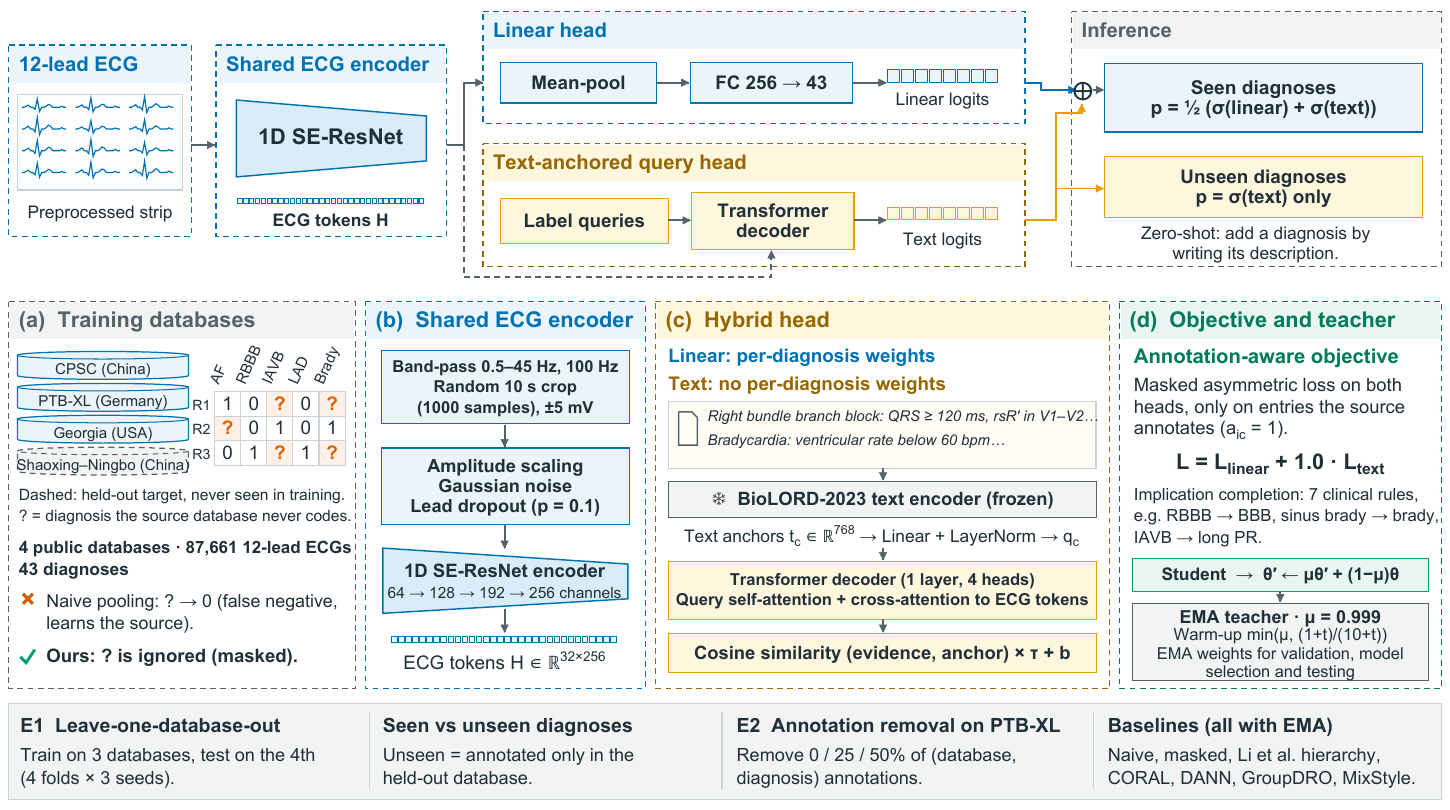
\includegraphics[width=\textwidth]{figures/fig_method_hybrid.png}}{\fbox{\parbox{0.9\textwidth}{\centering\vspace{2cm}Methodology figure (figures/fig\_method\_hybrid.pdf)\vspace{2cm}}}}}
\caption{Overview of the approach. (a) Training databases annotate different diagnosis vocabularies; an entry that a database never codes (``?'') is unknown, not negative, and naive pooling treats it as a negative. (b) A one-dimensional SE-ResNet encodes a 10\,s, 100\,Hz 12-lead recording into $T=32$ tokens. (c) Two heads read the same tokens: a linear head with one weight vector per diagnosis, and a text-anchored label-query head in which frozen clinical description embeddings (BioLORD-2023) act as queries that cross-attend to the tokens and are scored by cosine similarity, so that it has no diagnosis-specific weights. Diagnoses supervised in training are scored by the mean of the two probabilities; diagnoses never supervised are scored by the text head alone. (d) Both heads are trained with the same asymmetric loss restricted to source-annotated entries, after completion of positives through seven clinical implication rules; an exponential moving average of the weights is validated, selected and tested. The bottom strip lists the evaluation protocols.}\label{fig:method}
\end{figure}

\subsection{Overview}\label{sec:overview}
The method has four components, summarized in Table~\ref{tab:components}, each tied to one aspect of the problem. A one-dimensional residual encoder maps a 12-lead recording to a short sequence of tokens (Section~\ref{sec:encoder}). A \emph{hybrid head} reads these tokens twice (Section~\ref{sec:head}): a conventional linear head provides the discriminative capacity of per-diagnosis weights on diagnoses that the training sources annotate, and a text-anchored label-query head scores every diagnosis from a frozen embedding of its clinical description, so that diagnoses without any training label remain scorable (RQ3). An annotation-aware objective restricts the loss of both heads to entries that the record's source annotates and completes positives through implication rules (RQ1, Section~\ref{sec:objective}). Finally, model selection and inference use an exponential moving average of the weights, which stabilizes the selected model across the distribution shift between validation sources and the held-out database (RQ2, Section~\ref{sec:train}). Section~\ref{sec:why} formalizes why the naive pooled objective is misspecified and motivates the masked objective. Notation is summarized in Table~\ref{tab:notation}. The design was arrived at through a development process with selection rules fixed in advance; it is reported, with its negative intermediate results and one deviation from those rules, in Appendix~\ref{secA2}.

\begin{table}[!htbp]
\centering\footnotesize
\caption{Components of the method, the problem each addresses and where it is defined.}\label{tab:components}
\begin{tabularx}{\textwidth}{@{}l X X l@{}}
\toprule
Component & Problem addressed & Mechanism & Defined in \\
\midrule
ECG encoder & Variable-length, multi-rate recordings & Band-pass, 100\,Hz, random 10\,s crops; SE-ResNet tokens & Sec.~\ref{sec:encoder} \\
Linear head & Discriminative power on annotated diagnoses & Mean-pooled tokens, one weight vector per diagnosis & Eq.~\eqref{eq:linear} \\
Text-anchored head & Fixed label set; unseen diagnoses not scorable & Frozen description embeddings as queries; cosine scoring & Eqs.~\eqref{eq:query}--\eqref{eq:logit} \\
Score fusion & Combining both heads without losing open vocabulary & Mean probability on seen diagnoses, text head on unseen ones & Eq.~\eqref{eq:fusion} \\
Masked asymmetric loss & Unannotated entries treated as negatives & Loss on both heads, only on source-annotated entries & Eqs.~\eqref{eq:lann}--\eqref{eq:total} \\
Implication completion & Coarse findings implied but not coded & Seven child\,$\rightarrow$\,parent rules on targets & Eq.~\eqref{eq:rules} \\
Weight averaging & Unstable selection under source shift & EMA of weights with warm-up; EMA validated and tested & Eq.~\eqref{eq:ema} \\
\bottomrule
\end{tabularx}
\end{table}

\subsection{Problem formulation}\label{sec:problem}
Let $\mathcal{S}=\{1,\dots,S\}$ index the source databases and let $\mathcal{V}=\{1,\dots,C\}$ be a global diagnosis vocabulary. Source $s$ annotates a subset $\mathcal{V}_s\subseteq\mathcal{V}$; we define $\mathcal{V}_s$ operationally as the diagnoses with at least ten positive recordings in $s$ (Section~\ref{sec:data}). A training record is a tuple $(\mathbf{x}_i, \mathbf{y}_i, \mathbf{a}_i, s_i)$, where $\mathbf{x}_i\in\mathbb{R}^{12\times L}$ is a 12-lead ECG, $y_{ic}\in\{0,1\}$ indicates that diagnosis $c$ was coded, and $a_{ic}=\mathbbm{1}[c\in\mathcal{V}_{s_i}]$ indicates that $y_{ic}$ is \emph{observed}. When $a_{ic}=0$ the value $y_{ic}=0$ means ``not annotated'' rather than ``absent''. The goal is a scorer $p_c(\mathbf{x})\in[0,1]$ that performs well on a target database $s^\ast\notin\mathcal{S}$, both on the diagnoses that some training source annotates, $\mathcal{V}_{\mathrm{seen}}=\bigcup_{s\in\mathcal{S}}\mathcal{V}_s$, and on the diagnoses $\mathcal{V}_{s^\ast}\setminus\mathcal{V}_{\mathrm{seen}}$ that only the target annotates. We write $\kappa_c=\mathbbm{1}[c\in\mathcal{V}_{\mathrm{seen}}]$.

\begin{table}[!htbp]
\centering\footnotesize
\caption{Notation.}\label{tab:notation}
\begin{tabularx}{\textwidth}{@{}l X@{}}
\toprule
Symbol & Meaning \\
\midrule
$\mathcal{S}$, $S$ & Set and number of training source databases; $s^\ast$ is the held-out target database \\
$\mathcal{V}$, $C$ & Global diagnosis vocabulary and its size; $\mathcal{V}_s\subseteq\mathcal{V}$ the diagnoses annotated by source $s$ \\
$\mathbf{x}_i\in\mathbb{R}^{12\times L}$ & 12-lead recording $i$ at 100\,Hz; $L=1000$ for a 10\,s training crop \\
$y_{ic}\in\{0,1\}$ & Diagnosis $c$ coded for record $i$ \\
$a_{ic}\in\{0,1\}$ & Entry $(i,c)$ observed, i.e.\ $c\in\mathcal{V}_{s_i}$ \\
$\kappa_c\in\{0,1\}$ & Diagnosis $c$ annotated by at least one training source (seen) \\
$\mathbf{H}\in\mathbb{R}^{T\times D}$ & ECG token sequence from the encoder $f_\theta$; $T=32$, $D=256$ \\
$\bar{\mathbf{h}}\in\mathbb{R}^{D}$ & Mean of the $T$ tokens \\
$\mathbf{t}_c\in\mathbb{R}^{768}$ & Frozen text embedding (anchor) of the description of diagnosis $c$ \\
$\mathbf{q}_c\in\mathbb{R}^{D}$ & Label-specific evidence vector for diagnosis $c$ after the decoder \\
$\ell^{\mathrm{lin}}_c$, $\ell^{\mathrm{txt}}_c$ & Logits of diagnosis $c$ from the linear and the text-anchored head \\
$p_c$ & Reported probability for diagnosis $c$ (Eq.~\eqref{eq:fusion}) \\
$\tau$, $b$ & Learned scalar scale and bias of the text head \\
$\phi(\ell,y)$ & Asymmetric loss for one entry, as a function of the logit \\
$\theta$, $\bar\theta$ & Trained parameters and their exponential moving average; $\mu$ the EMA momentum \\
$\lambda_{\mathrm{txt}}$ & Weight of the text-head loss \\
$\mathcal{R}$ & Set of clinical implication rules $(c\rightarrow c')$ \\
$B$ & Mini-batch size \\
\bottomrule
\end{tabularx}
\end{table}

\subsection{Why naive pooling fails}\label{sec:why}
Naive pooling concatenates the databases and trains on the target $\tilde y_{ic}=y_{ic}a_{ic}$, so that every unannotated entry becomes a zero. The following proposition, a direct consequence of the well-known fact that cross-entropy is minimized by the conditional expectation of the target, makes explicit what such a model estimates. We state it for one diagnosis $c$ and drop the index.

\begin{proposition}\label{prop:naive}
Let $(\mathbf{x},y,a)$ be jointly distributed with $y,a\in\{0,1\}$, and let the model class be rich enough that the expected binary cross-entropy $\mathbb{E}[-\tilde y\log p(\mathbf{x})-(1-\tilde y)\log(1-p(\mathbf{x}))]$ can be minimized pointwise in $\mathbf{x}$. Then the naive minimizer is $p^\ast_{\mathrm{naive}}(\mathbf{x})=P(y=1,a=1\mid\mathbf{x})$, and the minimizer of the masked objective $\mathbb{E}[a\,(-y\log p(\mathbf{x})-(1-y)\log(1-p(\mathbf{x})))]$ is $p^\ast_{\mathrm{mask}}(\mathbf{x})=P(y=1\mid\mathbf{x},a=1)$ wherever $P(a=1\mid\mathbf{x})>0$. If, in addition, $y$ and $a$ are conditionally independent given $\mathbf{x}$, then
\begin{equation}
p^\ast_{\mathrm{naive}}(\mathbf{x})=P(y=1\mid\mathbf{x})\,P(a=1\mid\mathbf{x}),
\qquad
p^\ast_{\mathrm{mask}}(\mathbf{x})=P(y=1\mid\mathbf{x}).
\label{eq:prop}
\end{equation}
\end{proposition}

\begin{proof}
For a fixed $\mathbf{x}$ the naive risk is $-\eta\log p-(1-\eta)\log(1-p)$ with $\eta=\mathbb{E}[\tilde y\mid\mathbf{x}]=P(y=1,a=1\mid\mathbf{x})$, since $\tilde y=ya$ is a product of indicators; this function of $p\in(0,1)$ is minimized at $p=\eta$. For the masked risk, conditioning on $\mathbf{x}$ gives $P(a=1\mid\mathbf{x})\,[-\eta'\log p-(1-\eta')\log(1-p)]$ with $\eta'=\mathbb{E}[y\mid\mathbf{x},a=1]$, minimized at $p=\eta'$ whenever the prefactor is positive. Conditional independence factorizes $P(y=1,a=1\mid\mathbf{x})=P(y=1\mid\mathbf{x})P(a=1\mid\mathbf{x})$ and gives $P(y=1\mid\mathbf{x},a=1)=P(y=1\mid\mathbf{x})$.
\end{proof}

Two consequences follow. First, naive predictions are deflated by $P(a=1\mid\mathbf{x})$, the probability that the recording comes from a source that annotates $c$; a diagnosis coded by one of three sources is systematically under-scored. Second, and more harmful for cross-hospital use, $P(a=1\mid\mathbf{x})$ is a function of whatever distinguishes the sources in the signal, such as device, filtering and population characteristics. The naive objective therefore rewards recognizing the source, a shortcut that cannot transfer to a database the model has never seen. The masked objective removes this term, which is the role of $\Lann$ in Eq.~\eqref{eq:lann}.

\begin{remark}
Conditional independence of $y$ and $a$ given $\mathbf{x}$ is an idealization. Annotation depends on the source, and if the prevalence of $c$ differs between hospitals in a way that is not explained by the signal, then $P(y=1\mid\mathbf{x},a=1)$ is a source-conditional prevalence rather than $P(y=1\mid\mathbf{x})$, and even the masked objective inherits some source dependence. The masked objective also provides no signal at all on the entries with $a=0$, and in particular none on a diagnosis that no training source annotates. The text-anchored head addresses the latter case not by estimating the missing labels but by sharing parameters across diagnoses through their descriptions; an alternative that estimates them with teacher pseudo-labels was evaluated and is reported as an ablation (Section~\ref{sec:res_ablation}) and in Appendix~\ref{secA2}.
\end{remark}

\subsection{ECG encoder}\label{sec:encoder}
Recordings are band-pass filtered between 0.5\,Hz and $\min(45, f_s/2-1)$\,Hz with a second-order zero-phase Butterworth filter and resampled to 100\,Hz by polyphase filtering; the first 20\,s are stored and shorter recordings are zero-padded, with the number of valid samples retained. Training uses a random 10\,s window ($L=1000$) drawn inside the valid part of each record, and inference averages probabilities over 10\,s windows with a 5\,s stride (Section~\ref{sec:train}), so that findings within the first 20\,s of longer recordings are not lost; content beyond 20\,s (present only in CPSC) is discarded. Amplitudes are kept in millivolts and clipped to $\pm5$\,mV, without per-record normalization, because several diagnoses (for example low QRS voltage and ventricular hypertrophy) are defined by absolute amplitude. The encoder $f_\theta$ is a one-dimensional residual network with squeeze-and-excitation blocks~\cite{he2016,hu2018se}: a stem convolution (kernel 15, stride 2) with batch normalization and max-pooling is followed by four stages of two residual blocks (kernel 7, squeeze ratio 8) with widths $64,128,192,256$ and stage strides $1,2,2,2$. It maps $\mathbf{x}$ to a token sequence $\mathbf{H}=f_\theta(\mathbf{x})\in\mathbb{R}^{T\times D}$ with $T=32$ and $D=256$. All compared methods share this encoder.

\subsection{Hybrid label head}\label{sec:head}
\paragraph{Linear head.}
The linear head is the head used by every baseline: it averages the tokens, $\bar{\mathbf{h}}=\frac1T\sum_{t}\mathbf{H}_t$, and applies one affine map,
\begin{equation}
\boldsymbol{\ell}^{\mathrm{lin}}(\mathbf{x})=\mathbf{W}_{\mathrm{lin}}\bar{\mathbf{h}}+\mathbf{b}_{\mathrm{lin}},\qquad \mathbf{W}_{\mathrm{lin}}\in\mathbb{R}^{C\times D}.
\label{eq:linear}
\end{equation}
Each row of $\mathbf{W}_{\mathrm{lin}}$ belongs to one diagnosis; a row whose diagnosis is never observed in training receives no gradient and keeps its random initialization, so the linear head cannot score unseen diagnoses.

\paragraph{Text-anchored label-query head.}
Each diagnosis $c$ is described by a sentence $d_c$ that states its name and its standard ECG criteria, paraphrased from the AHA/ACCF/HRS recommendations~\cite{kligfield2007,surawicz2009} and written once before any experiment. For example, right bundle branch block is described as ``An ECG showing right bundle branch block. QRS duration of 120 ms or more with an rsR$'$ pattern in V1 and V2 and a wide slurred S wave in leads I and V6,'' first-degree atrioventricular block as ``An ECG showing first degree atrioventricular block. Every P wave is conducted to the ventricles but the PR interval is prolonged beyond 200 ms,'' and low QRS voltages as ``An ECG showing low QRS voltages. Small QRS amplitudes: peak-to-peak below 0.5 mV in all limb leads or below 1.0 mV in all precordial leads.'' The complete list is given in Supplementary Table~S1. A frozen biomedical sentence encoder, BioLORD-2023~\cite{remy_biolord}, maps each description to an anchor $\mathbf{t}_c\in\mathbb{R}^{768}$ once before training. Initial label queries are obtained by a linear projection followed by layer normalization,
\begin{equation}
\mathbf{q}^{(0)}_c=\mathrm{LN}(\mathbf{W}_q\mathbf{t}_c),
\label{eq:query}
\end{equation}
and a single pre-norm transformer decoder layer with four heads~\cite{liu2021q2l} applies self-attention among the $C$ queries and cross-attention from the queries to $\mathbf{H}+\mathbf{P}$, where $\mathbf{P}$ is a learned positional embedding, yielding label-specific evidence vectors $\mathbf{q}_c\in\mathbb{R}^{D}$. The text logit for diagnosis $c$ is the scaled cosine similarity between a projection of the evidence and a projection of the anchor,
\begin{equation}
\ell^{\mathrm{txt}}_c(\mathbf{x}) = \tau\,\big\langle \overline{\mathbf{W}_h\mathbf{q}_c},\ \overline{\mathbf{W}_g\mathbf{t}_c}\big\rangle + b,
\label{eq:logit}
\end{equation}
where $\overline{\mathbf{v}}=\mathbf{v}/\lVert\mathbf{v}\rVert$, and $\tau$ and $b$ are learned scalars shared by all diagnoses (initialized to 10 and $-2$). Because no parameter in Eqs.~\eqref{eq:query}--\eqref{eq:logit} is specific to a diagnosis, a diagnosis that was never supervised can be scored by writing its description and appending its anchor; whether this works in practice is an empirical question addressed in Section~\ref{sec:res_unseen}. During training, the queries of diagnoses that no training source annotates are present in the decoder but contribute no loss term.

\paragraph{Score fusion.}
At inference both heads are evaluated on the same tokens. A diagnosis that the training sources annotate is scored by the mean of the two probabilities, and a diagnosis that they do not annotate by the text head alone:
\begin{equation}
p_c(\mathbf{x})=
\begin{cases}
\tfrac12\big[\sigma(\ell^{\mathrm{lin}}_c(\mathbf{x}))+\sigma(\ell^{\mathrm{txt}}_c(\mathbf{x}))\big] & \text{if } \kappa_c=1,\\[2pt]
\sigma(\ell^{\mathrm{txt}}_c(\mathbf{x})) & \text{if } \kappa_c=0,
\end{cases}
\label{eq:fusion}
\end{equation}
where $\sigma$ is the logistic function. The partition $\kappa$ is known at training time from the annotation of the training sources and never uses the target. The rule follows from the roles of the two heads. On seen diagnoses the linear head has per-diagnosis weights that the text head lacks, while the text head contributes a differently parameterized estimate that shares statistical strength across related diagnoses; averaging two such estimates reduces variance in the same way as a two-member ensemble, at the cost of one shared encoder. On unseen diagnoses only the text head carries information, and the linear row is excluded because it is untrained. Two alternatives were evaluated as ablations: scoring seen diagnoses by the linear head alone, which keeps the text head as an auxiliary task only, and stopping the gradient of the text head into the encoder, which turns the hybrid into a post-hoc ensemble (Section~\ref{sec:res_ablation}).

Figure~\ref{fig:textsim} shows the cosine similarity between the anchors of the 26 scored diagnoses. Without any ECG data, the frozen encoder already places clinically related findings close together: conduction disturbances (right, incomplete right, left and unspecified bundle branch block), frontal-axis findings (left and right axis deviation, left anterior fascicular block), repolarization findings (T-wave abnormality and inversion), sinus-rate findings (sinus rhythm, sinus bradycardia, bradycardia) and atrioventricular conduction (first-degree block, prolonged PR interval; cosine 0.84). This structure is what allows supervision on one diagnosis to inform the queries of related diagnoses, including those a training database never annotates.

\begin{figure}[!htbp]
\centering
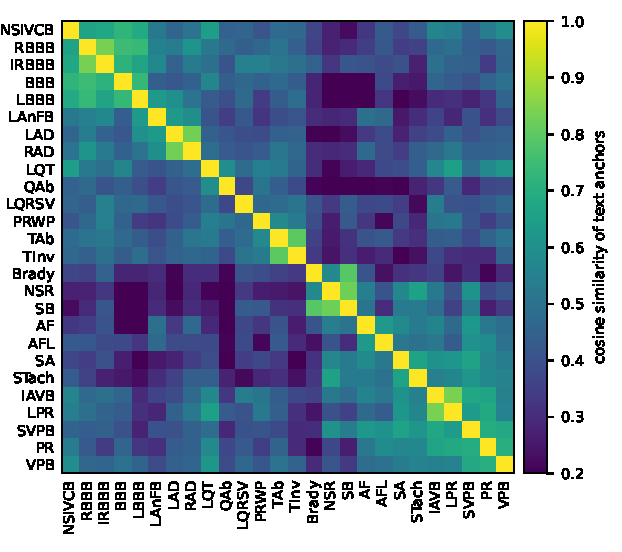
\includegraphics[width=0.78\textwidth]{figures/fig_text_similarity.pdf}
\caption{Cosine similarity between the frozen text anchors $\mathbf{t}_c$ (BioLORD-2023, full descriptions) of the 26 PhysioNet/CinC 2021 scored diagnoses (25 of them are in our vocabulary; poor R-wave progression does not occur in the four databases), ordered by average-linkage hierarchical clustering. Abbreviations follow Supplementary Table~S1.}\label{fig:textsim}
\end{figure}

\subsection{Annotation-aware objective}\label{sec:objective}
\paragraph{Masked asymmetric loss.}
With logit $\ell$, probability $p=\sigma(\ell)$ and target $y$, we use the asymmetric loss~\cite{ridnik_asl}
\begin{equation}
\phi(\ell,y) = -y\log p-(1-y)\,p_m^{\gamma}\log(1-p_m),\qquad p_m=\max(p-m,0),
\label{eq:asl}
\end{equation}
with $\gamma=2$ and $m=0.05$, which down-weights easy negatives in the strongly imbalanced multi-label setting. Only observed entries contribute, and each record is normalized by its number of observed entries so that records from sources with small vocabularies are not down-weighted. For a head with logits $\boldsymbol{\ell}$,
\begin{equation}
\Lann(\boldsymbol{\ell}) = \frac{1}{B}\sum_{i=1}^{B}\frac{\sum_{c} a_{ic}\,\phi\big(\ell_c(\mathbf{x}_i),y_{ic}\big)}{\max\big(1,\sum_c a_{ic}\big)} .
\label{eq:lann}
\end{equation}
Both heads are trained with the same targets and the same mask,
\begin{equation}
\mathcal{L}=\Lann(\boldsymbol{\ell}^{\mathrm{lin}})+\lambda_{\mathrm{txt}}\,\Lann(\boldsymbol{\ell}^{\mathrm{txt}}),\qquad \lambda_{\mathrm{txt}}=1,
\label{eq:total}
\end{equation}
so that the text head is a second, open-vocabulary reading of the same supervision and the encoder receives gradients from both. No term in $\mathcal{L}$ involves an unobserved entry.

\paragraph{Implication completion.}
A set $\mathcal{R}$ of seven clinical implication rules of the form child$\,\rightarrow\,$implied finding (Table~\ref{tab:rules}), for example right bundle branch block $\rightarrow$ bundle branch block, sinus bradycardia $\rightarrow$ bradycardia and first-degree atrioventricular block $\rightarrow$ prolonged PR interval, is applied to the training targets before the loss is computed:
\begin{equation}
y_{ic'}\leftarrow\max(y_{ic'},y_{ic}),\qquad a_{ic'}\leftarrow\max(a_{ic'},y_{ic'})\qquad\text{for }(c\rightarrow c')\in\mathcal{R},
\label{eq:rules}
\end{equation}
so that a completed positive is treated as observed even when the source never codes the implied finding. The rules encode clinical implication, not the SNOMED-CT \emph{is-a} hierarchy. Completion adds positives but never negatives, so a diagnosis that is supervised only through completion has positive-only supervision. Evaluation always uses the original, uncompleted labels.

\subsection{Training, weight averaging, inference and complexity}\label{sec:train}
Algorithm~\ref{alg:step} summarizes one training step. Models are trained for 30 epochs with AdamW (learning rate $10^{-3}$, weight decay $10^{-2}$), a one-cycle learning-rate schedule with 10\% warm-up, batch size $B=256$ and mixed precision; the last incomplete batch of each epoch is dropped. All methods share the random 10\,s crops, per-record amplitude scaling by a factor drawn from $U(0.8,1.2)$, additive Gaussian noise with standard deviation $0.02$\,mV, and lead dropout in which each lead is zeroed independently with probability $0.1$.

\paragraph{Weight averaging.}
After every optimization step $t$ an exponential moving average of the parameters is updated~\cite{tarvainen2017},
\begin{equation}
\bar\theta\leftarrow\mu_t\bar\theta+(1-\mu_t)\theta,\qquad \mu_t=\min\!\Big(\mu,\ \frac{1+t}{10+t}\Big),\quad \mu=0.999,
\label{eq:ema}
\end{equation}
where the warm-up of $\mu_t$ ensures that $\bar\theta$ does not retain a sizeable share of the random initialization during the first epochs (with a constant $\mu=0.999$, about a fifth of the initial weights would still be present after the first 1{,}600 steps). Batch-normalization statistics are copied rather than averaged. The averaged weights $\bar\theta$ are the ones that are validated after each epoch, selected, thresholded and tested. Weight averaging is applied identically to every baseline in our comparison, because in preliminary runs it improved all methods, and leaving it out of the baselines would have confounded the comparison (Appendix~\ref{secA2}).

\paragraph{Model selection and thresholds.}
After every epoch the averaged model is evaluated on a validation split drawn from the training sources, and the checkpoint with the highest macro AUROC over the diagnoses evaluable in that split is retained. Validation AUROC and the F1 thresholds are computed only over observed entries of the original, uncompleted labels: for each diagnosis, over the validation records whose source annotates it, so that model selection does not reward treating unknown entries as negatives. Per-diagnosis decision thresholds are chosen on the same split to maximize F1 over a grid from 0.02 to 0.98 in steps of 0.02. The target database is never used for model selection or threshold tuning. At inference each record is scored by averaging the probabilities of Eq.~\eqref{eq:fusion} over all 10\,s windows at a 5\,s stride that fall inside its valid part.

\paragraph{Complexity.}
The text head adds, per record, self-attention over $C$ queries and cross-attention from $C$ queries to $T$ tokens, i.e.\ $\mathcal{O}(C^2D+CTD)$ operations, which for $C=43$ and $T=32$ is small relative to the convolutional encoder. The hybrid model has 4.62\,M trainable parameters: 3.35\,M in the encoder, 11\,k in the linear head and 1.27\,M in the text-anchored head; the baselines have 3.36\,M (encoder and linear head). The frozen text encoder is used only once, offline, to compute the anchors, so the deployed model needs no language model. A training run on the leave-one-database-out protocol takes a median of 12 minutes on a single cloud GPU, against 10 minutes for the masked baseline.

\begin{algorithm}[!htbp]
\caption{One training step of the proposed method.}\label{alg:step}
\begin{algorithmic}[1]
\Require mini-batch $\{(\mathbf{x}_i,\mathbf{y}_i,\mathbf{a}_i)\}_{i=1}^{B}$ with completed targets (Eq.~\eqref{eq:rules}); anchors $\{\mathbf{t}_c\}$; parameters $\theta$; averaged parameters $\bar\theta$; step $t$
\State $\mathbf{x}^{\mathrm{c}}_i \gets \textsc{RandomCrop}_{10\,\mathrm{s}}(\mathbf{x}_i)$ for all $i$ \Comment{inside the valid part of each record}
\State $\mathbf{x}^{\mathrm{a}}_i \gets \textsc{Augment}(\mathbf{x}^{\mathrm{c}}_i)$ \Comment{amplitude scaling, noise, lead dropout}
\State $\mathbf{H}_i \gets f_\theta(\mathbf{x}^{\mathrm{a}}_i)$ \Comment{shared tokens}
\State $\boldsymbol{\ell}^{\mathrm{lin}}_i \gets \mathbf{W}_{\mathrm{lin}}\bar{\mathbf{h}}_i+\mathbf{b}_{\mathrm{lin}}$;\quad $\boldsymbol{\ell}^{\mathrm{txt}}_i \gets \textsc{TextHead}(\mathbf{H}_i,\{\mathbf{t}_c\})$ \Comment{Eqs.~\eqref{eq:linear}--\eqref{eq:logit}}
\State $\mathcal{L}\gets\Lann(\boldsymbol{\ell}^{\mathrm{lin}})+\lambda_{\mathrm{txt}}\Lann(\boldsymbol{\ell}^{\mathrm{txt}})$ \Comment{Eqs.~\eqref{eq:lann}, \eqref{eq:total}; observed entries only}
\State $\theta\gets\textsc{AdamW}(\theta,\nabla_\theta\mathcal{L})$; advance the one-cycle schedule
\State $\mu_t\gets\min(\mu,(1+t)/(10+t))$;\quad $\bar\theta\gets\mu_t\bar\theta+(1-\mu_t)\theta$ \Comment{Eq.~\eqref{eq:ema}}
\end{algorithmic}
\end{algorithm}

%=====================================================================
\section{Experimental setup}\label{sec:setup}
%=====================================================================

\subsection{Data}\label{sec:data}
We use four public 12-lead databases from three countries (Table~\ref{tab:datasets}, Fig.~\ref{fig:demo}): the China Physiological Signal Challenge 2018 database together with its extra set (CPSC2018 and CPSC-Extra, pooled as ``CPSC'')~\cite{liu_cpsc2018,perez2020}, PTB-XL from Germany~\cite{wagner2020}, the Georgia 12-lead ECG Challenge database from the United States~\cite{perez2020}, and the Shaoxing and Ningbo First Hospital database from China~\cite{zheng2020,zheng2022ningbo}, as redistributed by the PhysioNet/CinC 2021 Challenge~\cite{reyna2022} and hosted on PhysioNet~\cite{goldberger2000}. The two further Challenge sources, the St.~Petersburg INCART database (long Holter recordings) and the original PTB database, are too small to serve as held-out targets and are excluded. CPSC comprises two releases of one challenge and Shaoxing--Ningbo pools two hospitals released together; we therefore speak of databases rather than hospitals. Diagnoses are SNOMED-CT codes from the record headers; the four code equivalences defined by the 2021 Challenge are applied to all methods before anything else (Table~\ref{tab:rules}). Records shorter than 5\,s, flat records and duplicates are discarded during preprocessing, which removes two recordings and leaves 87{,}661 recordings in the four databases. All recordings were acquired at 500\,Hz; PTB-XL, Georgia and Shaoxing--Ningbo recordings last at most 10\,s, whereas CPSC recordings last 6--144\,s (median 12\,s).

The global vocabulary $\mathcal{V}$ consists of the diagnoses for which a clinical description was written (Supplementary Table~S1) and which have at least 50 positive recordings across the four databases and at least ten in one of them; it contains $C=43$ diagnoses, of which 25 belong to the 26 classes scored in the 2021 Challenge and the remainder are frequent unscored codes. A database \emph{annotates} a diagnosis when it has at least ten positive recordings of it. Table~\ref{tab:datasets} reports the size of each annotated vocabulary, Fig.~\ref{fig:annot} shows the full coverage pattern, and Supplementary Table~S2 gives the full database-by-diagnosis count matrix. All counts are computed from the output of the preprocessing script and are not edited by hand.

\begin{table}[t]\centering\footnotesize\setlength{\tabcolsep}{4pt}
\caption{Databases used in this study after excluding recordings shorter than 5\,s, flat recordings and duplicates (two recordings in total). All recordings were sampled at 500\,Hz. Duration in seconds, median (range). Age excludes missing values and the PTB-XL anonymization code (300) used for patients older than 89 years. Annotated = number of vocabulary diagnoses with at least ten positive recordings in the database.}\label{tab:datasets}
\begin{tabular*}{\textwidth}{@{\extracolsep{\fill}}llrcccr@{}}\toprule
Database & Country & Records & Duration (s) & Age (years) & Female (\%) & Annotated \\ \midrule
CPSC & China & 10,328 & 12 (6--144) & 61.4 $\pm$ 18.0 & 46.3 & 24 \\
PTB-XL & Germany & 21,837 & 10 (10--10) & 59.5 $\pm$ 16.8 & 47.9 & 32 \\
Georgia & USA & 10,344 & 10 (5--10) & 60.5 $\pm$ 15.4 & 46.3 & 33 \\
Shaoxing--Ningbo & China & 45,152 & 10 (10--10) & 58.2 $\pm$ 19.7 & 43.6 & 41 \\
\midrule Total & & 87,661 & & & & 43 \\
\bottomrule\end{tabular*}\end{table}


\begin{figure}[!htbp]
\centering
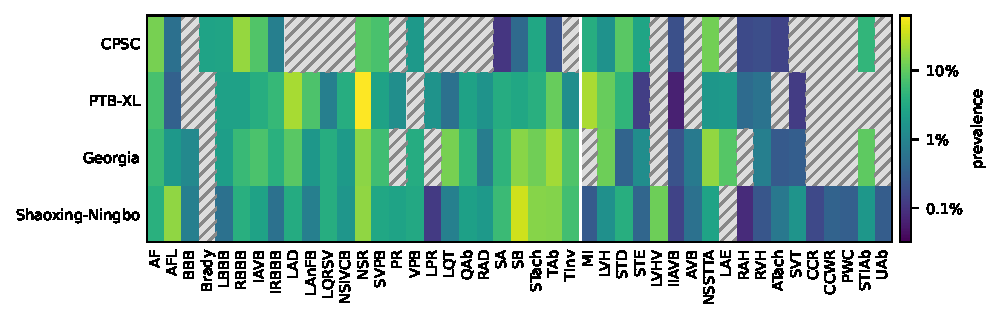
\includegraphics[width=\textwidth]{figures/fig_annotation_matrix.pdf}
\caption{Annotation coverage of the four databases over the $C=43$ vocabulary diagnoses. Colour gives the prevalence of each diagnosis in each database on a logarithmic scale; hatched cells mark diagnoses that the database does not annotate (fewer than ten positive recordings). Only 18 of the 43 diagnoses are annotated by all four databases, and 16.7\% of all record--diagnosis entries in the pooled label matrix are unknown rather than negative. Under naive pooling every hatched cell is treated as a confirmed negative.}\label{fig:annot}
\end{figure}

\begin{figure}[!htbp]
\centering
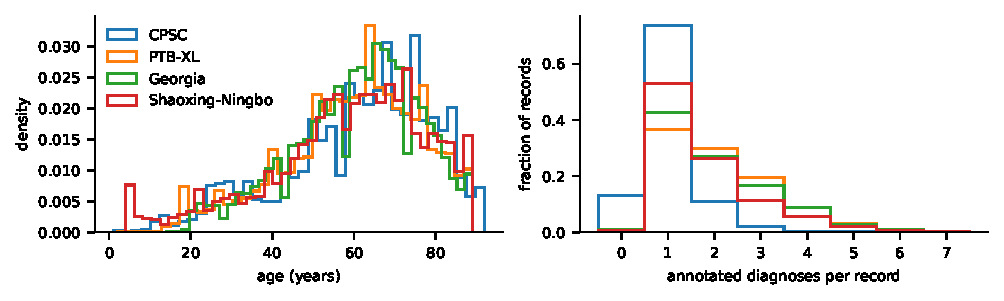
\includegraphics[width=\textwidth]{figures/fig_demographics.pdf}
\caption{Population characteristics of the four databases. Ages above 89 years are coded as 300 in PTB-XL for anonymity and are excluded from the age statistics.}\label{fig:demo}
\end{figure}


\subsection{Protocols}\label{sec:protocols}
\paragraph{E1: leave-one-database-out.}
Each of the four databases is held out in turn. The model is trained on the pooled records of the other three, of which a fixed random 10\% (split seed 0) serves as the validation split for model selection and threshold tuning, and tested on all records of the held-out database, restricted to the diagnoses that database annotates. Diagnoses annotated by at least one training source are reported as \emph{seen}; those annotated only by the held-out database are \emph{unseen}. The partition and the indicator $\kappa_c$ are computed from the raw annotation rule before implication completion, so it is a property of the fold, not of the method. Two folds have evaluable unseen diagnoses: CPSC (bradycardia, one diagnosis) and Shaoxing--Ningbo (left ventricular high voltage, clockwise and counterclockwise cardiac rotation, P-wave change and abnormal U wave; five diagnoses). Bradycardia is the implied finding of the rule sinus bradycardia $\rightarrow$ bradycardia, so every method that uses implication completion receives positive-only supervision for it when CPSC is held out; the five Shaoxing--Ningbo diagnoses receive no supervision of any kind. Unseen diagnoses can be scored meaningfully only by models without diagnosis-specific weights; we nevertheless report the linear-head baselines on them, whose untrained rows provide an empirical chance reference.

\paragraph{E2: controlled annotation removal.}
To isolate the effect of the objective from that of the data, we simulate heterogeneous annotation on a single database. PTB-XL records are split at random into 80\% training, 10\% validation and 10\% test (patient identifiers are not included in the Challenge redistribution, so the split is by record). Each diagnosis that PTB-XL annotates is then removed from the training supervision independently with probability $r\in\{0,0.25,0.5\}$ (sinus rhythm is protected), as if PTB-XL had never coded it: the corresponding targets become zero and the corresponding entries become unobserved. The removed diagnoses are drawn once per rate with a fixed seed, from the raw annotation and before implication completion, and are shared by all methods; at $r=0.25$ seven diagnoses are removed and at $r=0.5$ seventeen (listed in Supplementary Table~S4). Naive pooling, the Li-style baseline and the proposed method are trained on the altered supervision and evaluated against the complete original labels, separately over the retained and the removed diagnoses. A removed diagnosis is annotated by no training record, so for the proposed method it is an unseen diagnosis scored by the text head, while for the baselines its linear row receives only negative targets (naive) or no gradient at all (Li-style), unless an implication rule completes it. Because a single source offers no source shortcut, E2 isolates the effect of label handling from that of distribution shift.

\paragraph{E3: systematic zero-shot evaluation.}
E1 contains only six genuinely unseen diagnoses, in two folds. To evaluate open-vocabulary scoring on a broad and pre-specified set of diagnoses, E3 withholds diagnoses that would normally be seen. In each leave-one-database-out fold, every diagnosis that the held-out database annotates and that at least one training source annotates (sinus rhythm excepted) is assigned to one of 4--6 fixed groups of about six diagnoses, drawn at random once (seed 0) and listed in Supplementary Table~S5. Each run withholds one group: its columns are removed from the raw labels \emph{before} implication completion, so that no trained diagnosis is completed from a withheld one, and they never enter the loss. The withheld diagnoses are then scored on the held-out database by the text head alone. Every eligible diagnosis is thus scored zero-shot exactly once per fold and seed, giving 120 (database, diagnosis) pairs over four folds, each with three seeds (60 training runs). For each pair we compare the zero-shot AUROC with chance, with the AUROC that the same model obtains when the diagnosis is trained (from E1), and with the zero-shot AUROC of a report-pretrained ECG--language model (Section~\ref{sec:baselines}). We also test whether zero-shot accuracy depends on the cosine similarity between the description anchor of the withheld diagnosis and the nearest anchor of a trained diagnosis.

\paragraph{Annotation threshold and calibration.}
The proposed method and the Li-style baseline are re-run on all folds (seed 0) with the annotation threshold set to 5 and to 20 positives instead of 10; both the vocabulary and the annotated sets change accordingly. Calibration on seen diagnoses is assessed for all methods from the E1 test predictions by the expected calibration error (15 equal-width bins), the Brier score and the ratio of mean predicted probability to observed prevalence; no method is recalibrated.

\paragraph{Ablations.}
Four variants of the proposed method, run under E1 with three seeds, change one design decision each: (i) \emph{linear scoring} scores seen diagnoses by the linear head alone, so the text head acts only as an auxiliary training task on the shared encoder and as the scorer of unseen diagnoses; (ii) \emph{detached text head} stops the gradient of the text-head loss into the encoder, so that the encoder is trained exactly as in the Li-style baseline and the hybrid reduces to a post-hoc ensemble of two heads; (iii) \emph{+ pseudo-labels} adds soft pseudo-labels from the averaged model on unobserved entries of seen diagnoses, applied to the text head from the third epoch; and (iv) \emph{text head only} is the strongest single-head text-anchored model from our development sweep, in which a class-specific residual (bias, query read-out and pooled read-out for seen diagnoses) is added to the text logit and soft pseudo-labels with soft implication consistency are used (Appendix~\ref{secA2}). A second group of seven single-seed ablations of an earlier text-only model (learned instead of text queries, name-only descriptions, a general-domain text encoder, removal of implication completion, of MixStyle or of the text head) is reported in Appendix~\ref{secA2}.

\subsection{Baselines}\label{sec:baselines}
All baselines share the encoder, preprocessing, augmentation including lead dropout, loss function, optimizer, schedule, weight averaging and model-selection rule of the proposed method; they differ only in how labels and sources are handled, and all use the linear head of Eq.~\eqref{eq:linear}. \textbf{Naive pooling} treats every unannotated entry as a negative. \textbf{Masked} ignores unannotated entries (Eq.~\eqref{eq:lann}). \textbf{Li-style} combines masking with implication-based completion of the targets, following the prediction-masking and category-mapping idea of Li et al.~\cite{li2024}; it is a re-implementation of that label handling within our shared training framework, not their original code or architecture. The proposed method uses exactly the Li-style label handling, so the comparison between the two isolates the effect of the hybrid head. The domain-generalization (DG) baselines add one of the following to the Li-style configuration: \textbf{CORAL}~\cite{sun2016coral}, a penalty on the squared difference between the covariance matrices of the mean-pooled encoder features of each pair of sources (weight 1.0); \textbf{DANN}~\cite{ganin2016}, a two-layer source classifier on the mean-pooled features trained through a gradient-reversal layer (weight 0.1); \textbf{GroupDRO}~\cite{sagawa2020}, an exponentiated-gradient reweighting of the per-source losses (step size 0.01); and \textbf{MixStyle}~\cite{zhou2021mixstyle}, which mixes channel-wise feature means and standard deviations between recordings after the first two encoder stages (probability 0.5, mixing weights from $\mathrm{Beta}(0.1,0.1)$). The DG loss weights were fixed before any experiment to the values above and were not tuned; we return to this in Section~\ref{sec:limitations}. Every baseline is trained, like the proposed method, with weight averaging (Eq.~\eqref{eq:ema}); weight averaging improved every baseline in preliminary single-seed runs (Appendix~\ref{secA2}), so omitting it would have weakened the comparison.

For zero-shot scoring we compare against \textbf{MERL}~\cite{merl2024}, an ECG--language model pretrained on several hundred thousand MIMIC-IV-ECG recordings paired with their free-text reports, using the authors' released code and ResNet-18 checkpoint with the MedCPT text encoder, strictly zero-shot: no training or fine-tuning on any of our data. Our band-passed 100\,Hz windows are upsampled to MERL's 500\,Hz input, the leads are reordered to its convention, each window is min--max normalized as in MERL's preprocessing, and cosine scores are averaged over the same 10\,s windows as for our models. MERL is evaluated with its own clinical-knowledge-enhanced prompts, with our descriptions and with bare class names, on the same held-out databases and diagnoses. Its released checkpoint was selected on validation splits of PTB-XL, CPSC2018 and Chapman--Shaoxing, which overlap with three of our held-out databases; this can only favour MERL.

\subsection{Method selection protocol}\label{sec:selection}
The configuration of the proposed method was chosen on validation data by a rule written down before the candidates were trained: candidate configurations were trained on one fold (Georgia held out, seed 0), the candidate with the highest validation macro AUROC on the \emph{source} validation split was selected, and ties within 0.001 were broken in favour of the simpler configuration. The four hybrid candidates were linear scoring, mean-probability scoring, the detached text head and mean-probability scoring with pseudo-labels. Their validation AUROCs were 0.9519, 0.9527, 0.9533 and 0.9523; the detached variant was within 0.001 of mean-probability scoring and therefore not preferred, so mean-probability scoring was selected. The same rule also recorded the validation AUROC of the strongest baseline on the same fold (Li-style with weight averaging, 0.9531), and the selected configuration did \emph{not} exceed it on validation, which shows that the test-set advantage of Section~\ref{sec:res_seen} was not anticipated by the selection data. For this case the rule specified a fallback to linear scoring, which met its conditions (0.9519, within 0.002 of the reference); we did not apply the fallback and kept mean-probability scoring. This is a deviation from the pre-registered rule. It was made before the remaining folds and seeds were run, but the sweep result files also contained the Georgia seed-0 test metrics of the candidates, which were visible at the time (H1 85.43, H2 85.70); the choice can therefore not be regarded as blind to test data on that one fold and seed. Both configurations were run on all folds with three seeds, and Appendix~\ref{secA2:hybrid} discusses how the conclusions would change under the fallback. All other folds and seeds of the proposed method, all baselines and all ablations were run afterwards with the frozen configuration. The complete development history, including an earlier text-only design that underperformed the baselines, is given in Appendix~\ref{secA2}.

\subsection{Implementation details}\label{sec:impl}
Table~\ref{tab:hyper} lists every hyper-parameter. All values were fixed before the main experiments and shared across folds and methods; none was tuned on a held-out database. Each run uses a single cloud GPU (NVIDIA Tesla P100 or T4 on Kaggle, or A100 on Google Colab); results do not depend on the GPU type beyond floating-point non-determinism. In E1, every method and every ablation of the hybrid model is run with three seeds (0, 1, 2) on all four folds, giving twelve runs per method; seeds vary the weight initialization and batch order while the data split is fixed. E2 and the threshold sensitivity use a single seed, and E3 three seeds. In total the paper reports 229 training runs (153 for E1, E2 and the ablations, 60 for E3 and 16 for the threshold analysis), plus MERL inference.

\begin{table}[!htbp]
\centering\footnotesize
\caption{Hyper-parameters. All values are shared by every method unless stated otherwise.}\label{tab:hyper}
\begin{tabularx}{\textwidth}{@{}l l X@{}}
\toprule
Group & Parameter & Value \\
\midrule
\multirow{5}{*}{Preprocessing}
 & Band-pass filter & 0.5--$\min(45,f_s/2-1)$\,Hz, 2nd-order Butterworth, zero-phase \\
 & Sampling rate; stored length & 100\,Hz; first 20\,s (zero-padded if shorter) \\
 & Amplitude & millivolts, clipped to $\pm5$\,mV, no per-record normalization \\
 & Vocabulary rule & $\ge50$ positives in total and $\ge10$ in one database \\
 & Annotation rule & $\ge10$ positives in the database \\
\midrule
\multirow{4}{*}{Augmentation (all methods)}
 & Training crop & random 10\,s window inside the valid part \\
 & Amplitude scaling & factor $\sim U(0.8,1.2)$ per record \\
 & Additive noise & Gaussian, $\sigma=0.02$\,mV \\
 & Lead dropout & each lead zeroed with probability 0.1 \\
\midrule
\multirow{4}{*}{Encoder}
 & Stem & conv (kernel 15, stride 2), BN, ReLU, max-pool (3, stride 2) \\
 & Stages & 4 stages $\times$ 2 SE-residual blocks, kernel 7, SE ratio 8 \\
 & Widths; strides & 64, 128, 192, 256; 1, 2, 2, 2 \\
 & Output & $T=32$ tokens of dimension $D=256$ \\
\midrule
\multirow{4}{*}{Text-anchored head}
 & Text encoder & BioLORD-2023 (frozen), 768-d anchors \\
 & Decoder & 1 pre-norm layer, 4 heads, feed-forward 512, dropout 0.1 \\
 & Positional embedding & learned, up to 64 tokens \\
 & Scale $\tau$; bias $b$ & learned scalars, initialized to 10 and $-2$ \\
\midrule
\multirow{5}{*}{Objective}
 & Asymmetric loss & $\gamma=2$, $m=0.05$ \\
 & Loss mask & observed entries only, after implication completion (7 rules) \\
 & Text-head loss weight $\lambda_{\mathrm{txt}}$ & 1.0 (hybrid only) \\
 & Weight averaging (all methods) & EMA, $\mu=0.999$, warm-up $\min(\mu,(1+t)/(10+t))$, every step \\
 & Seen-diagnosis score (hybrid) & mean of the linear and text-head probabilities \\
\midrule
\multirow{4}{*}{Optimization}
 & Optimizer & AdamW, learning rate $10^{-3}$, weight decay $10^{-2}$ \\
 & Schedule & one-cycle, 10\% warm-up, 30 epochs \\
 & Batch size; precision & 256 (last incomplete batch dropped); mixed precision \\
 & Model selection & best validation macro AUROC of the averaged weights over epochs \\
\midrule
\multirow{4}{*}{DG baselines}
 & CORAL weight & 1.0 \\
 & MixStyle & $p=0.5$, $\mathrm{Beta}(0.1,0.1)$, after stages 1 and 2 \\
 & DANN weight; reversal factor & 0.1; 1.0 \\
 & GroupDRO step size & 0.01 \\
\midrule
\multirow{3}{*}{Inference and evaluation}
 & Windows & 10\,s, stride 5\,s, mean probability \\
 & Thresholds & grid 0.02--0.98 (step 0.02), max F1 on validation \\
 & Evaluable diagnosis & annotated in the evaluated database with $\ge5$ positives \\
\bottomrule
\end{tabularx}
\end{table}

\subsection{Metrics and statistics}\label{sec:metrics}
Primary metrics are macro-averaged AUROC and area under the precision--recall curve (AUPRC) over the diagnoses that the evaluated database annotates and that have at least five positive recordings in the evaluated records. Both are threshold-free; AUROC is additionally invariant to prevalence, whereas the AUPRC baseline equals prevalence, so AUPRC is compared between methods within a database but not across databases. The five-positive rule matters only for the validation split and the E2 test split, since in E1 every annotated diagnosis has at least ten positives in the held-out database. We additionally report macro F1 at the thresholds tuned on the source validation split and, as an upper bound that no deployed system could reach, an oracle F1 at the best threshold on the target. We report mean and standard deviation over the three seeds.

Statistical comparisons are made at two levels, each with Holm's correction within a pre-defined family. (i) \emph{Across folds and seeds}, the primary analysis: for each baseline, the twelve paired differences (four folds $\times$ three seeds) in macro AUROC, and separately in macro AUPRC, between the proposed method and the baseline are tested with the exact two-sided Wilcoxon signed-rank test; the family is the seven baselines per metric. This analysis treats training randomness and the choice of held-out database as the sources of variation. (ii) \emph{Within a fold}: differences in macro AUROC between the seed-0 runs are tested with a paired bootstrap over test records (2{,}000 resamples), from which we report the difference, its 95\% confidence interval and a two-sided $p$-value; the family is all four folds $\times$ seven baselines. This analysis treats the test records as the source of variation. Per-diagnosis AUROC differences between the proposed method and the strongest baseline of each fold are tested with DeLong's test~\cite{delong1988}, with Holm's correction over all per-diagnosis tests. Unseen-diagnosis and E2 results are reported descriptively. Every number in the tables is produced by aggregation scripts from the logged run files, and the mapping from each cell to its source run is recorded.

%=====================================================================
\section{Results}\label{sec:results}
%=====================================================================
All numbers in this section are produced by the aggregation scripts from the logged run files of the 153 training runs (Section~\ref{sec:impl}); means and standard deviations are over three seeds unless stated otherwise.

\subsection{Seen diagnoses under leave-one-database-out}\label{sec:res_seen}
Table~\ref{tab:loso} reports macro AUROC and AUPRC over seen diagnoses for each held-out database and each method, and Fig.~\ref{fig:seeds} shows every individual run. Averaged over the four held-out databases, the proposed method obtains the highest macro AUROC ($86.6_{\pm0.1}$) and the highest macro AUPRC ($33.0_{\pm0.2}$) of all methods. The strongest baselines are the two label-handling methods without a domain-generalization component, masked loss and Li-style masking ($86.3$ each), followed by the four DG methods ($86.1$ for CORAL, GroupDRO and MixStyle; $85.6$ for DANN) and naive pooling ($85.6$). The ordering of the baselines already illustrates the first part of RQ1: ignoring unannotated entries instead of treating them as negatives raises macro AUROC by 0.7 points and AUPRC by 0.6 points, and none of the DG penalties improves on masking alone.

\IfFileExists{generated/tab_loso.tex}{\begin{sidewaystable}
\centering
\footnotesize
\setlength{\tabcolsep}{3pt}
\caption{Leave-one-database-out results: macro AUROC and AUPRC ($\times 100$) over labels seen in training, mean$_{\pm\mathrm{std}}$ over seeds where more than one seed is available. Best per column in bold.}
\label{tab:loso}
\begin{tabular}{lcccccccccc}
\toprule
 & \multicolumn{2}{c}{CPSC} & \multicolumn{2}{c}{PTB-XL} & \multicolumn{2}{c}{Georgia} & \multicolumn{2}{c}{Shaoxing-Ningbo} & \multicolumn{2}{c}{Mean} \\
\cmidrule(lr){2-3} \cmidrule(lr){4-5} \cmidrule(lr){6-7} \cmidrule(lr){8-9} \cmidrule(lr){10-11}
Method & AUROC & AUPRC & AUROC & AUPRC & AUROC & AUPRC & AUROC & AUPRC & AUROC & AUPRC \\
\midrule
Naive (unknown = negative) & 84.4$_{\pm 0.5}$ & 26.4$_{\pm 0.2}$ & 86.7$_{\pm 0.3}$ & 37.7$_{\pm 0.4}$ & 84.6$_{\pm 0.2}$ & 35.9$_{\pm 0.2}$ & 86.7$_{\pm 0.4}$ & 29.1$_{\pm 0.2}$ & 85.6$_{\pm 0.2}$ & 32.3$_{\pm 0.2}$ \\
Masked loss & 84.4$_{\pm 0.5}$ & 26.8$_{\pm 0.2}$ & 87.3$_{\pm 0.4}$ & 38.2$_{\pm 0.5}$ & 85.5$_{\pm 0.2}$ & \textbf{36.4}$_{\pm 0.1}$ & 88.1$_{\pm 0.2}$ & 30.2$_{\pm 0.2}$ & 86.3$_{\pm 0.2}$ & 32.9$_{\pm 0.1}$ \\
Hierarchical mask (Li et al.) & 84.2$_{\pm 0.2}$ & 26.8$_{\pm 0.2}$ & 87.6$_{\pm 0.2}$ & \textbf{38.7}$_{\pm 0.3}$ & \textbf{85.6}$_{\pm 0.1}$ & 35.8$_{\pm 0.3}$ & 87.7$_{\pm 0.1}$ & 29.8$_{\pm 0.4}$ & 86.3$_{\pm 0.1}$ & 32.8$_{\pm 0.3}$ \\
CORAL & 84.4$_{\pm 0.4}$ & 25.9$_{\pm 0.1}$ & 87.5$_{\pm 0.1}$ & 38.2$_{\pm 0.5}$ & 85.1$_{\pm 0.2}$ & 35.0$_{\pm 0.3}$ & 87.5$_{\pm 0.5}$ & 29.4$_{\pm 0.7}$ & 86.1$_{\pm 0.1}$ & 32.1$_{\pm 0.2}$ \\
DANN & 84.1$_{\pm 0.2}$ & 26.4$_{\pm 0.4}$ & 86.8$_{\pm 0.4}$ & 38.0$_{\pm 0.3}$ & 84.7$_{\pm 0.3}$ & 35.0$_{\pm 0.3}$ & 86.8$_{\pm 0.5}$ & 28.4$_{\pm 0.3}$ & 85.6$_{\pm 0.2}$ & 32.0$_{\pm 0.2}$ \\
GroupDRO & \textbf{84.8}$_{\pm 0.1}$ & \textbf{27.7}$_{\pm 0.5}$ & 87.3$_{\pm 0.2}$ & 37.5$_{\pm 0.3}$ & 84.8$_{\pm 0.0}$ & 34.1$_{\pm 0.1}$ & 87.5$_{\pm 0.1}$ & 29.9$_{\pm 0.5}$ & 86.1$_{\pm 0.1}$ & 32.3$_{\pm 0.1}$ \\
MixStyle & 84.4$_{\pm 0.3}$ & 26.4$_{\pm 0.2}$ & 87.4$_{\pm 0.1}$ & 38.1$_{\pm 0.1}$ & 85.3$_{\pm 0.1}$ & 35.2$_{\pm 0.2}$ & 87.2$_{\pm 0.7}$ & 29.3$_{\pm 0.5}$ & 86.1$_{\pm 0.1}$ & 32.2$_{\pm 0.1}$ \\
\midrule
Ours & 84.5$_{\pm 0.2}$ & 27.2$_{\pm 0.2}$ & \textbf{87.9}$_{\pm 0.2}$ & 38.6$_{\pm 0.4}$ & 85.6$_{\pm 0.1}$ & 35.8$_{\pm 0.3}$ & \textbf{88.3}$_{\pm 0.3}$ & \textbf{30.4}$_{\pm 0.5}$ & \textbf{86.6}$_{\pm 0.1}$ & \textbf{33.0}$_{\pm 0.2}$ \\
\bottomrule
\end{tabular}
\end{sidewaystable}
}{}

\begin{figure}[!htbp]
\centering
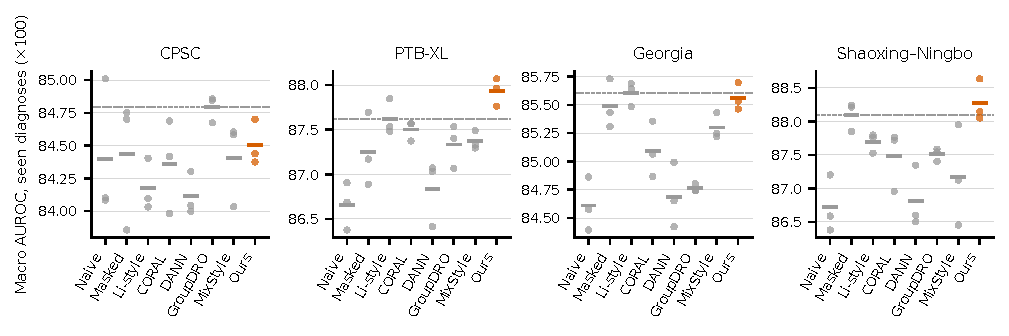
\includegraphics[width=\textwidth]{generated/fig_seen_seeds.pdf}
\caption{Seen-diagnosis macro AUROC of every run, per held-out database. Dots are individual seeds, horizontal bars the mean over three seeds; the dashed line marks the best baseline mean of each database. The proposed method (orange) has the highest mean on PTB-XL and Shaoxing--Ningbo, is level with the best baseline on Georgia, and lies within the spread of the baselines on CPSC.}\label{fig:seeds}
\end{figure}

The advantage is not uniform across databases. It is largest on PTB-XL ($87.9$ against $87.6$ for the best baseline) and Shaoxing--Ningbo ($88.3$ against $88.1$), where the mean of the proposed method exceeds that of every baseline (Fig.~
ef{fig:seeds}). On Georgia the proposed method ties with Li-style masking ($85.6$), and on CPSC it lies within the spread of the baselines, GroupDRO being highest ($84.8$ against $84.5$). CPSC is the held-out database with the smallest annotated vocabulary and the longest recordings, and GroupDRO, which up-weights the worst-performing source, is the only DG method that helps on it.

Table~\ref{tab:seedstats} gives the primary statistical analysis over the twelve paired fold--seed runs. For macro AUROC, the proposed method is better than every baseline in at least eight of twelve pairs; after Holm correction the difference is significant against six of the seven baselines (naive, Li-style, CORAL, DANN, GroupDRO and MixStyle; $p_{\mathrm{Holm}}\le0.014$) but not against the masked baseline (mean difference $+0.25$ points, eight of twelve pairs, $p=0.052$). For macro AUPRC, the difference is significant against naive pooling, CORAL, DANN and MixStyle, but not against masked loss, Li-style or GroupDRO. The proposed method therefore matches the strongest baseline on seen diagnoses and significantly improves on the domain-generalization methods, with an effect size of a few tenths of a point of AUROC; it does not establish a significant advantage over well-implemented masking. Because our pre-specified selection rule would have chosen the linear-scoring variant rather than mean-probability fusion (Section~\ref{sec:selection}), we also report that variant here: its mean seen-diagnosis AUROC is $86.06_{\pm0.19}$, 0.21 points below the Li-style baseline, and its unseen-diagnosis AUROC is the same as that of the selected configuration (Table~\ref{tab:ablation}). Under the pre-specified rule, the conclusion on seen diagnoses would therefore be ``on par with or slightly below the strongest baselines'' rather than ``on par with the strongest and significantly above the others''; all conclusions on unseen and removed diagnoses are unaffected.

\begin{table}[!htbp]
\centering\footnotesize
\setlength{\tabcolsep}{4pt}
\caption{Primary statistical comparison over the twelve paired runs (four held-out databases $\times$ three seeds) of seen-diagnosis macro AUROC and AUPRC ($\times100$): mean difference (ours $-$ baseline), number of pairs in which the proposed method is better, and the exact two-sided Wilcoxon signed-rank $p$, Holm-adjusted over the seven baselines within each metric. Bold: $p_{\mathrm{Holm}}<0.05$.}\label{tab:seedstats}
\begin{tabular}{lcccccc}
\toprule
 & \multicolumn{3}{c}{Macro AUROC} & \multicolumn{3}{c}{Macro AUPRC} \\
\cmidrule(lr){2-4}\cmidrule(lr){5-7}
Ours vs. & $\Delta$ & wins & $p_{\mathrm{Holm}}$ & $\Delta$ & wins & $p_{\mathrm{Holm}}$ \\
\midrule
Naive pooling & $+0.97$ & 11/12 & \textbf{0.009} & $+0.75$ & 9/12 & \textbf{0.049} \\
Masked loss & $+0.25$ & 8/12 & 0.052 & $+0.15$ & 7/12 & 0.380 \\
Li-style & $+0.30$ & 10/12 & \textbf{0.010} & $+0.23$ & 8/12 & 0.105 \\
CORAL & $+0.46$ & 11/12 & \textbf{0.009} & $+0.92$ & 12/12 & \textbf{0.003} \\
DANN & $+0.95$ & 12/12 & \textbf{0.003} & $+1.07$ & 12/12 & \textbf{0.003} \\
GroupDRO & $+0.47$ & 9/12 & \textbf{0.014} & $+0.71$ & 10/12 & 0.081 \\
MixStyle & $+0.51$ & 11/12 & \textbf{0.010} & $+0.79$ & 12/12 & \textbf{0.003} \\
\bottomrule
\end{tabular}
\end{table}

The within-fold bootstrap of Table~\ref{tab:stats} gives the same picture from the perspective of test-record sampling. Of the 28 comparisons of the seed-0 runs, 15 remain significant after Holm correction, all in favour of the proposed method: five on PTB-XL, four on Georgia and six on Shaoxing--Ningbo; no comparison is significant on CPSC, and none is significant in favour of a baseline. Against the masked baseline, the difference is significant on PTB-XL ($+0.9$ points, 95\% CI $[0.4,1.4]$) but not on the other three folds.

\IfFileExists{generated/tab_stats.tex}{\begin{sidewaystable}
\centering
\footnotesize
\setlength{\tabcolsep}{3pt}
\caption{Paired bootstrap (2000 resamples of test records) of the difference in macro AUROC ($\times 100$) between our method and each baseline (seed 0), with 95\% confidence interval and two-sided $p$ (Holm-adjusted over all comparisons in the table). Bottom: number of labels for which our method is significantly better / worse than the strongest baseline per target (DeLong test, Holm-adjusted $p<0.05$) out of all evaluated labels.}
\label{tab:stats}
\begin{tabular}{lcccccccc}
\toprule
 & \multicolumn{2}{c}{CPSC} & \multicolumn{2}{c}{PTB-XL} & \multicolumn{2}{c}{Georgia} & \multicolumn{2}{c}{Shaoxing-Ningbo} \\
\cmidrule(lr){2-3} \cmidrule(lr){4-5} \cmidrule(lr){6-7} \cmidrule(lr){8-9}
Ours vs. & $\Delta$ [95\% CI] & $p_\mathrm{Holm}$ & $\Delta$ [95\% CI] & $p_\mathrm{Holm}$ & $\Delta$ [95\% CI] & $p_\mathrm{Holm}$ & $\Delta$ [95\% CI] & $p_\mathrm{Holm}$ \\
\midrule
Naive (unknown = negative) & $+0.3$ [-0.3, 0.9] & 1.000 & $+0.9$ [0.5, 1.2] & 0.028 & $+0.8$ [0.5, 1.2] & 0.028 & $+0.9$ [0.6, 1.0] & 0.028 \\
Masked loss & $+0.6$ [-0.3, 1.3] & 1.000 & $+0.9$ [0.4, 1.4] & 0.028 & $-0.0$ [-0.3, 0.2] & 1.000 & $+0.2$ [0.0, 0.4] & 0.325 \\
Hierarchical mask (Li et al.) & $+0.4$ [-0.3, 1.1] & 1.000 & $+0.3$ [-0.0, 0.6] & 0.550 & $+0.2$ [-0.0, 0.4] & 0.550 & $+0.5$ [0.4, 0.7] & 0.028 \\
CORAL & $+0.5$ [-0.3, 1.2] & 1.000 & $+0.4$ [0.0, 0.8] & 0.325 & $+0.3$ [0.0, 0.6] & 0.325 & $+0.3$ [0.1, 0.5] & 0.032 \\
DANN & $+0.4$ [-0.4, 1.1] & 1.000 & $+1.3$ [0.9, 1.8] & 0.028 & $+1.3$ [1.0, 1.6] & 0.028 & $+1.5$ [1.2, 1.7] & 0.028 \\
GroupDRO & $-0.2$ [-1.1, 0.5] & 1.000 & $+0.7$ [0.3, 1.1] & 0.028 & $+0.9$ [0.6, 1.1] & 0.028 & $+0.5$ [0.3, 0.7] & 0.028 \\
MixStyle & $-0.2$ [-1.0, 0.5] & 1.000 & $+0.4$ [0.2, 0.7] & 0.032 & $+0.4$ [0.2, 0.7] & 0.042 & $+1.6$ [1.4, 1.8] & 0.028 \\
\midrule
DeLong vs.\ best & \multicolumn{2}{c}{GroupDRO: 3 / 1 of 23} & \multicolumn{2}{c}{Hierarchical mask (Li et al.): 1 / 4 of 32} & \multicolumn{2}{c}{Masked loss: 3 / 2 of 33} & \multicolumn{2}{c}{Masked loss: 7 / 5 of 36} \\
\bottomrule
\end{tabular}
\end{sidewaystable}
}{}

Table~\ref{tab:loso_f1} reports macro F1. At thresholds tuned on the source validation split all methods lie between $28.2$ and $29.7$ on average, and the proposed method ($29.4$) is not distinguishable from the best label-handling baselines; at the oracle threshold it obtains the highest mean F1 ($37.9$). The gap of about eight points between source-tuned and oracle F1, which is similar for all methods, shows that decision thresholds transfer poorly between databases whatever the training method, a point we return to in Section~\ref{sec:discussion}.

\IfFileExists{generated/tab_loso_f1.tex}{\begin{sidewaystable}
\centering
\footnotesize
\setlength{\tabcolsep}{3pt}
\caption{Leave-one-database-out macro F1 ($\times 100$) over seen labels, with thresholds tuned on source validation data (F1) and the oracle threshold on the target (F1$^{*}$, upper bound).}
\label{tab:loso_f1}
\begin{tabular}{lcccccccccc}
\toprule
 & \multicolumn{2}{c}{CPSC} & \multicolumn{2}{c}{PTB-XL} & \multicolumn{2}{c}{Georgia} & \multicolumn{2}{c}{Shaoxing-Ningbo} & \multicolumn{2}{c}{Mean} \\
\cmidrule(lr){2-3} \cmidrule(lr){4-5} \cmidrule(lr){6-7} \cmidrule(lr){8-9} \cmidrule(lr){10-11}
Method & F1 & F1$^{*}$ & F1 & F1$^{*}$ & F1 & F1$^{*}$ & F1 & F1$^{*}$ & F1 & F1$^{*}$ \\
\midrule
Naive (unknown = negative) & 23.4$_{\pm 0.4}$ & 32.1$_{\pm 0.3}$ & 31.2$_{\pm 0.6}$ & 41.5$_{\pm 0.3}$ & 32.1$_{\pm 0.6}$ & 41.1$_{\pm 0.4}$ & 26.1$_{\pm 0.5}$ & 33.5$_{\pm 0.4}$ & 28.2$_{\pm 0.4}$ & 37.1$_{\pm 0.1}$ \\
Masked loss & 23.8$_{\pm 0.1}$ & 32.6$_{\pm 0.2}$ & 32.4$_{\pm 0.7}$ & 42.2$_{\pm 0.2}$ & \textbf{33.4}$_{\pm 0.6}$ & \textbf{41.4}$_{\pm 0.1}$ & \textbf{28.3}$_{\pm 0.2}$ & 34.6$_{\pm 0.3}$ & 29.5$_{\pm 0.2}$ & 37.7$_{\pm 0.1}$ \\
Hierarchical mask (Li et al.) & 23.9$_{\pm 0.4}$ & 32.6$_{\pm 0.4}$ & 32.9$_{\pm 1.1}$ & 42.4$_{\pm 0.2}$ & 33.1$_{\pm 0.9}$ & 41.1$_{\pm 0.2}$ & 28.1$_{\pm 0.9}$ & 34.3$_{\pm 0.4}$ & 29.5$_{\pm 0.5}$ & 37.6$_{\pm 0.3}$ \\
CORAL & 23.7$_{\pm 0.5}$ & 31.7$_{\pm 0.2}$ & 32.8$_{\pm 0.8}$ & 42.1$_{\pm 0.3}$ & 33.0$_{\pm 0.5}$ & 40.0$_{\pm 0.4}$ & 27.5$_{\pm 0.3}$ & 34.1$_{\pm 0.7}$ & 29.3$_{\pm 0.2}$ & 37.0$_{\pm 0.2}$ \\
DANN & 23.8$_{\pm 0.5}$ & 31.8$_{\pm 0.4}$ & 32.7$_{\pm 1.2}$ & 41.8$_{\pm 0.3}$ & 33.3$_{\pm 1.0}$ & 39.9$_{\pm 0.4}$ & 26.8$_{\pm 0.8}$ & 33.3$_{\pm 0.1}$ & 29.2$_{\pm 0.4}$ & 36.7$_{\pm 0.2}$ \\
GroupDRO & \textbf{25.6}$_{\pm 0.4}$ & \textbf{33.3}$_{\pm 0.5}$ & \textbf{32.9}$_{\pm 0.7}$ & 41.1$_{\pm 0.4}$ & 32.0$_{\pm 0.3}$ & 38.9$_{\pm 0.1}$ & 28.2$_{\pm 0.5}$ & 34.4$_{\pm 0.3}$ & \textbf{29.7}$_{\pm 0.3}$ & 36.9$_{\pm 0.1}$ \\
MixStyle & 24.1$_{\pm 0.3}$ & 32.3$_{\pm 0.3}$ & 32.7$_{\pm 1.1}$ & 41.8$_{\pm 0.2}$ & 32.8$_{\pm 0.4}$ & 40.5$_{\pm 0.1}$ & 27.7$_{\pm 0.4}$ & 34.0$_{\pm 0.4}$ & 29.3$_{\pm 0.3}$ & 37.2$_{\pm 0.1}$ \\
\midrule
Ours & 23.8$_{\pm 0.4}$ & 33.1$_{\pm 0.5}$ & 32.9$_{\pm 0.2}$ & \textbf{42.5}$_{\pm 0.2}$ & 33.0$_{\pm 0.9}$ & 41.2$_{\pm 0.3}$ & 27.8$_{\pm 0.4}$ & \textbf{34.7}$_{\pm 0.5}$ & 29.4$_{\pm 0.2}$ & \textbf{37.9}$_{\pm 0.3}$ \\
\bottomrule
\end{tabular}
\end{sidewaystable}
}{}

\subsection{Unseen diagnoses}\label{sec:res_unseen}
Table~\ref{tab:unseen} and Fig.~\ref{fig:unseen} report the AUROC on diagnoses that only the held-out database annotates. On Shaoxing--Ningbo, where five diagnoses (left ventricular high voltage, clockwise and counterclockwise rotation, P-wave change and abnormal U wave) received no supervision of any kind, the proposed method obtains a macro AUROC of $67.0_{\pm1.3}$, against 51.2--53.2 for the seven baselines, whose untrained linear rows score at chance as expected. Four of the five diagnoses are scored clearly above chance by the text head: left ventricular high voltage ($71.3$, 5{,}401 positives), clockwise rotation ($73.3$), abnormal U wave ($74.8$) and P-wave change ($60.6$); counterclockwise rotation is close to chance ($54.9$). On CPSC the single unseen diagnosis, bradycardia, is implied by sinus bradycardia, so every method with implication completion has positive-only supervision for it; Li-style masking and the DG methods built on it reach 89.4--89.8 (CORAL 70.7, DANN 49.2), whereas the masked and naive baselines, which do not complete the label, remain at 48.0 and 64.6. The proposed method reaches $94.3_{\pm0.2}$, 4.5 points above the best baseline, which shows that the text anchor turns positive-only supervision into a well-ranked score where a linear row cannot.

\begin{table}[!htbp]
\centering\footnotesize
\setlength{\tabcolsep}{4pt}
\caption{AUROC ($\times100$) on diagnoses annotated only by the held-out database (unseen), mean$_{\pm\mathrm{std}}$ over three seeds. CPSC: bradycardia (1 diagnosis; supervised positive-only through implication completion by methods that use it). Shaoxing--Ningbo: macro AUROC over five diagnoses without any supervision. Linear-head baselines score unseen diagnoses with untrained or positive-only rows and serve as a chance reference.}\label{tab:unseen}
\begin{tabular}{lcc}
\toprule
Method & CPSC (Brady) & Shaoxing--Ningbo (5 diagnoses) \\
\midrule
Naive pooling & $64.6_{\pm1.2}$ & $53.2_{\pm4.6}$ \\
Masked loss & $48.0_{\pm1.3}$ & $52.1_{\pm1.5}$ \\
Li-style & $89.4_{\pm0.2}$ & $51.3_{\pm6.1}$ \\
CORAL & $70.7_{\pm4.4}$ & $51.8_{\pm0.6}$ \\
DANN & $49.2_{\pm12.7}$ & $52.6_{\pm3.0}$ \\
GroupDRO & $89.8_{\pm0.3}$ & $52.6_{\pm6.9}$ \\
MixStyle & $89.5_{\pm0.3}$ & $51.2_{\pm3.3}$ \\
\midrule
Ours (hybrid; text head on unseen) & $\mathbf{94.3}_{\pm0.2}$ & $\mathbf{67.0}_{\pm1.3}$ \\
\bottomrule
\end{tabular}
\end{table}

\begin{figure}[!htbp]
\centering
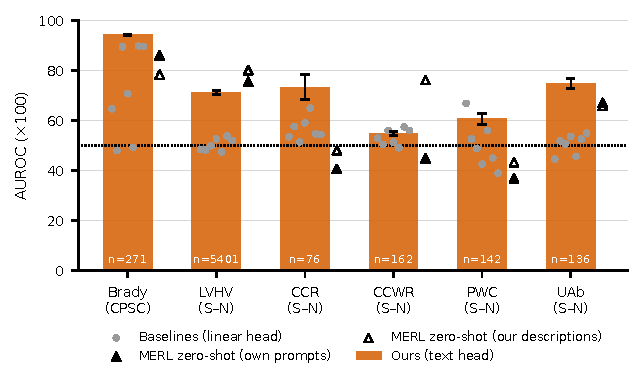
\includegraphics[width=0.75\textwidth]{generated/fig_unseen.pdf}
\caption{AUROC on each unseen diagnosis, mean over three seeds (bars, error bars one standard deviation) for the text head of the proposed method, and the seven linear-head baselines (grey dots). $n$ is the number of positive recordings in the held-out database. The dotted line marks chance. Abbreviations: Brady bradycardia; LVHV left ventricular high voltage; CCR, CCWR clockwise and counterclockwise cardiac rotation; PWC P-wave change; UAb abnormal U wave; S--N Shaoxing--Ningbo.}\label{fig:unseen}
\end{figure}

\subsection{Controlled annotation removal}\label{sec:res_e2}
Table~\ref{tab:e2} and Fig.~\ref{fig:e2} report the PTB-XL annotation-removal experiment. With complete annotation ($r=0$) the three methods are within 0.1 points of each other ($94.0$--$94.1$), confirming that the hybrid head does not cost in-distribution accuracy. When annotation is removed, the retained diagnoses degrade only mildly for all methods (at $r=0.5$: naive $92.6$, Li-style $91.3$, ours $93.1$). The removed diagnoses separate the methods. The linear baselines score them at or below chance: naive pooling $47.1$ and $55.5$ at $r=0.25$ and $0.5$, and Li-style $55.8$ and $47.6$, with large diagnosis-to-diagnosis variation that reflects the arbitrary orientation of untrained or negative-only rows. The proposed method scores them at $66.6$ and $69.0$, i.e.\ its open-vocabulary performance does not decline when the number of removed diagnoses grows from seven to seventeen. Per diagnosis at $r=0.5$ (Fig.~\ref{fig:e2}, right), the text head recovers conduction findings almost completely (right bundle branch block $93.5$, left anterior fascicular block $94.4$, first-degree AV block $78.2$, prolonged PR $73.8$), as well as atrial fibrillation ($77.2$) and flutter ($87.1$), T-wave inversion ($82.5$) and nonspecific ST--T abnormality ($82.1$). It fails on findings whose description is close to that of a related but different finding: sinus tachycardia ($43.6$), right axis deviation ($37.7$) and low QRS voltages ($49.6$). Over all diagnoses, removing annotation lowers the macro AUROC of the proposed method from $94.0$ to $79.5$ at $r=0.5$, against $71.6$ for naive pooling and $66.5$ for Li-style.

\begin{table}[!htbp]
\centering\footnotesize
\setlength{\tabcolsep}{5pt}
\caption{Controlled annotation removal on PTB-XL (single seed): macro AUROC ($\times100$) on the retained and the removed diagnoses and over all diagnoses, at removal rate $r$. At $r=0.25$ seven and at $r=0.5$ seventeen diagnoses are removed.}\label{tab:e2}
\begin{tabular}{lccccccc}
\toprule
 & $r=0$ & \multicolumn{3}{c}{$r=0.25$} & \multicolumn{3}{c}{$r=0.5$} \\
\cmidrule(lr){2-2}\cmidrule(lr){3-5}\cmidrule(lr){6-8}
Method & all & retained & removed & all & retained & removed & all \\
\midrule
Naive pooling & 94.1 & 93.2 & 47.1 & 82.5 & 92.6 & 55.5 & 71.6 \\
Li-style & 94.1 & 93.2 & 55.8 & 84.4 & 91.3 & 47.6 & 66.5 \\
Ours & 94.0 & 92.5 & \textbf{66.6} & \textbf{86.5} & \textbf{93.1} & \textbf{69.1} & \textbf{79.5} \\
\bottomrule
\end{tabular}
\end{table}

\begin{figure}[!htbp]
\centering
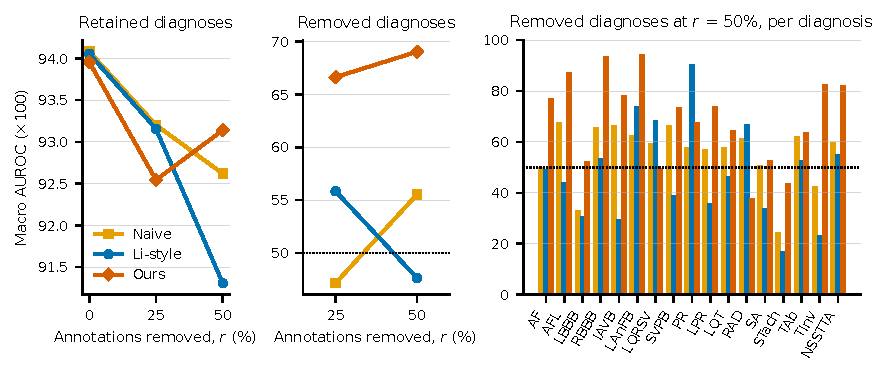
\includegraphics[width=\textwidth]{generated/fig_e2.pdf}
\caption{Controlled annotation removal on PTB-XL. Left and centre: macro AUROC on the retained and the removed diagnoses as a function of the fraction $r$ of PTB-XL diagnoses removed from training supervision. Right: AUROC on each of the seventeen diagnoses removed at $r=0.5$. The dotted line marks chance. Abbreviations follow Supplementary Table~S1.}\label{fig:e2}
\end{figure}

\subsection{Ablations}\label{sec:res_ablation}
Table~\ref{tab:ablation} and Fig.~\ref{fig:ablation} compare the selected configuration with the four variants of Section~\ref{sec:protocols}, all with three seeds, together with the Li-style baseline, which has the same label handling and encoder but no text head. Three observations follow. First, the gain on seen diagnoses comes from \emph{fusing} the two heads, not from the text head as an auxiliary task: scoring seen diagnoses by the linear head alone (linear scoring) gives $86.06$, slightly below the Li-style baseline ($86.27$), so jointly training the text head does not by itself improve the linear head. Second, joint training helps the fused model: the detached variant, which is a post-hoc ensemble of a Li-style encoder with a text head, reaches $86.43$, and letting the text-head gradient reach the encoder adds a further $0.14$ points ($86.57$), with the lowest seed variance of all configurations ($\pm0.07$). Third, adding pseudo-labels (86.38) and replacing the hybrid by the best text-only design (85.66) both reduce performance; the text-only model also scores unseen diagnoses worse ($62.0$ against $67.0$), so the linear head improves the text head through the shared encoder as well. All hybrid variants score unseen Shaoxing--Ningbo diagnoses between $66.5$ and $67.3$, so the unseen-diagnosis performance is a property of the text head and is robust to how seen diagnoses are scored.

\begin{table}[!htbp]
\centering\scriptsize
\setlength{\tabcolsep}{1pt}
\caption{Ablations of the hybrid model under leave-one-database-out (three seeds each): seen-diagnosis macro AUROC per held-out database and mean, mean AUPRC, and macro AUROC on the five unseen Shaoxing--Ningbo diagnoses ($\times100$, mean$_{\pm\mathrm{std}}$). The Li-style baseline has the same label handling and encoder without a text head.}\label{tab:ablation}
\begin{tabular}{lccccccc}
\toprule
 & \multicolumn{4}{c}{Seen AUROC} & \multicolumn{2}{c}{Seen, mean} & Unseen \\
\cmidrule(lr){2-5}\cmidrule(lr){6-7}\cmidrule(lr){8-8}
Configuration & CPSC & PTB-XL & Georgia & S--N & AUROC & AUPRC & S--N \\
\midrule
Li-style (no text head) & 84.2$_{\pm 0.2}$ & 87.6$_{\pm 0.2}$ & 85.6$_{\pm 0.1}$ & 87.7$_{\pm 0.1}$ & 86.27$_{\pm 0.15}$ & 32.8$_{\pm 0.3}$ & 51.3$_{\pm 6.1}$ \\
\textbf{Ours} (fusion) & 84.5$_{\pm 0.2}$ & 87.9$_{\pm 0.2}$ & 85.6$_{\pm 0.1}$ & \textbf{88.3}$_{\pm 0.3}$ & \textbf{86.57}$_{\pm 0.07}$ & \textbf{33.0}$_{\pm 0.2}$ & 67.0$_{\pm 1.3}$ \\
(i) Linear scoring & 84.3$_{\pm 0.2}$ & 87.4$_{\pm 0.1}$ & 85.2$_{\pm 0.2}$ & 87.4$_{\pm 0.6}$ & 86.06$_{\pm 0.19}$ & 32.4$_{\pm 0.3}$ & \textbf{67.3}$_{\pm 0.8}$ \\
(ii) Detached text head & 84.1$_{\pm 0.1}$ & \textbf{88.0}$_{\pm 0.2}$ & \textbf{85.7}$_{\pm 0.1}$ & 88.0$_{\pm 0.1}$ & 86.43$_{\pm 0.05}$ & 32.8$_{\pm 0.1}$ & 66.7$_{\pm 1.0}$ \\
(iii) + pseudo-labels & \textbf{84.6}$_{\pm 0.1}$ & 87.6$_{\pm 0.1}$ & 85.5$_{\pm 0.1}$ & 87.9$_{\pm 0.3}$ & 86.38$_{\pm 0.09}$ & 32.9$_{\pm 0.2}$ & 66.5$_{\pm 0.1}$ \\
(iv) Text head only & 83.9$_{\pm 0.2}$ & 86.6$_{\pm 0.0}$ & 84.8$_{\pm 0.6}$ & 87.3$_{\pm 0.1}$ & 85.66$_{\pm 0.19}$ & 32.0$_{\pm 0.2}$ & 62.0$_{\pm 1.7}$ \\
\bottomrule
\end{tabular}
\end{table}

\begin{figure}[!htbp]
\centering
\IfFileExists{generated/fig_ablation.pdf}{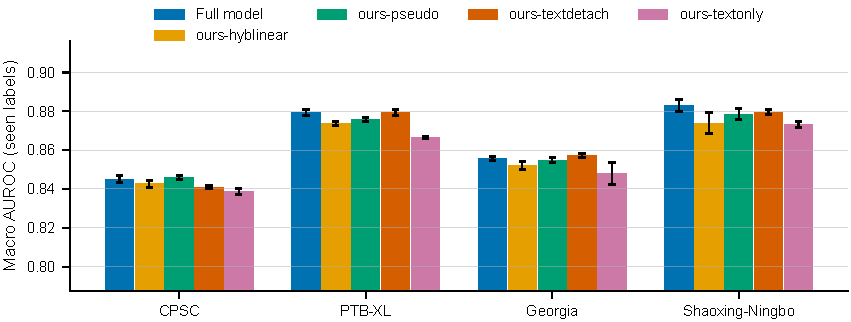
\includegraphics[width=\textwidth]{generated/fig_ablation.pdf}}{}
\caption{Seen-diagnosis macro AUROC of the selected configuration (``Full model'') and the four ablations per held-out database; bars are means over three seeds and error bars one standard deviation. ours-hyblinear: linear scoring; ours-textdetach: detached text head; ours-pseudo: with pseudo-labels; ours-textonly: text head only.}\label{fig:ablation}
\end{figure}

\subsection{Per-diagnosis analysis}\label{sec:res_perlabel}
Figure~\ref{fig:heatmap} shows, for each held-out database and each evaluable seen diagnosis, the AUROC difference between the proposed method and the strongest baseline of that database (seed 0), with DeLong tests Holm-corrected over all per-diagnosis comparisons; the bottom row of Table~\ref{tab:stats} counts the significant differences. The differences are small for most diagnoses and go in both directions: the proposed method is significantly better on 14 of 124 database--diagnosis pairs and significantly worse on 12, which is consistent with a two-head ensemble that redistributes rather than uniformly raises per-diagnosis accuracy. The largest gains are on conduction and morphology findings that share their description with related diagnoses (for example bundle branch block on Georgia, $+12.2$ points, and atrial flutter and nonspecific intraventricular conduction disorder on Shaoxing--Ningbo, $+5.7$ and $+6.6$), and the largest losses are on diagnoses defined by an absolute amplitude or interval that the description cannot convey precisely (low QRS voltages on Shaoxing--Ningbo, $-2.8$, and prolonged QT on Georgia, $-3.5$), and on bundle branch block on Shaoxing--Ningbo ($-7.8$). The sign of the bundle-branch-block difference thus depends on the database, which indicates that this parent finding is coded differently across sources.

\begin{figure}[!htbp]
\centering
\IfFileExists{generated/fig_perlabel_heatmap.pdf}{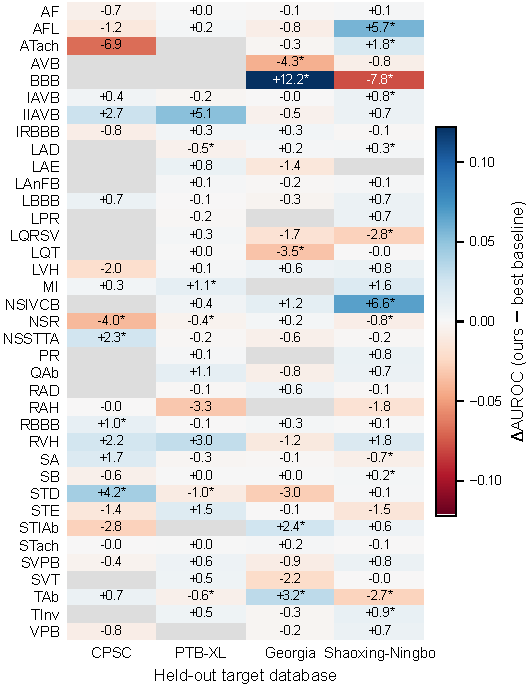
\includegraphics[width=\textwidth]{generated/fig_perlabel_heatmap.pdf}}{}
\caption{Per-diagnosis AUROC difference (proposed method $-$ strongest baseline of each held-out database, seed 0, $\times100$) on seen diagnoses. Marked cells are significant by DeLong's test after Holm correction over all per-diagnosis tests. Empty cells: diagnosis not evaluable in that database.}\label{fig:heatmap}
\end{figure}

%=====================================================================
\section{Discussion}\label{sec:discussion}
%=====================================================================

\subsection{Principal findings}\label{sec:disc_findings}
\paragraph{RQ1: learning from heterogeneous annotation.}
Treating unannotated entries as unknown rather than negative is the single most effective change for seen diagnoses: masked loss improves on naive pooling by 0.7 points of macro AUROC and 0.6 points of AUPRC (Table~\ref{tab:loso}), and in the controlled experiment the masked objective keeps retained diagnoses within 2.8 points of their complete-annotation accuracy while half of the annotation is removed (Table~\ref{tab:e2}). This is the behaviour predicted by Proposition~\ref{prop:naive}. On top of correct label handling, the hybrid head adds a further, small but consistent improvement: it has the highest mean AUROC and AUPRC of all methods, is better than every baseline in at least eight of twelve fold--seed pairs, and the difference is significant against six of the seven baselines. It is not significant against the masked baseline, and we do not claim that the hybrid head improves seen-diagnosis accuracy over well-implemented masking; the defensible statement is that it matches the best label-handling baseline on seen diagnoses while adding capabilities that no baseline has.

\paragraph{RQ2: transfer to an unseen database.}
None of the four domain-generalization methods improved on masking alone, and DANN was the weakest method after naive pooling. This agrees with the observation that DG penalties tuned for one benchmark rarely help consistently across held-out domains~\cite{ballas2022}, and it suggests that, in pooled public ECG data, the label-induced shortcut of Proposition~\ref{prop:naive} is a larger source of transfer error than the feature-statistics differences that DG methods target. Within each held-out database, the hybrid model is significantly better than most baselines on PTB-XL, Georgia and Shaoxing--Ningbo, but not on CPSC, whose small and rhythm-centred vocabulary leaves the least room for a text head that shares information between related diagnoses. Weight averaging, which we applied to all methods, improved every baseline by 0.3--1.8 points (Appendix~\ref{secA2}); it is an inexpensive component that published multi-source ECG comparisons should include in all arms.

\paragraph{RQ3: scoring diagnoses without labels.}
The clearest result of the study concerns diagnoses for which no training label exists. On the five Shaoxing--Ningbo diagnoses that no training database annotates, the text head reaches a macro AUROC of 67.0, against chance for every baseline, and on bradycardia, which the training data supervise only through an implication rule, it reaches 94.3 against 89.8 for the best linear head. In the controlled experiment, removed PTB-XL diagnoses are scored at 66.6--69.0 by the text head and at or below chance by the baselines, and per-diagnosis results show near-complete recovery of conduction and rhythm findings whose descriptions are close to those of supervised diagnoses (right bundle branch block 93.5, left anterior fascicular block 94.4, atrial flutter 87.1). The systematic evaluation E3 shows that this is not a property of a few favourable diagnoses: over 120 withheld diagnosis--database pairs, the text head scores 88\% above chance with a macro AUROC of 70.2, retaining on average 63\% of the above-chance AUROC that full supervision reaches. These are not clinically adequate accuracies for most diagnoses, but they are obtained without a single label, from a model whose seen-diagnosis accuracy is unchanged. Zero-shot accuracy increases with the semantic proximity between the description and the nearest trained diagnosis ($\rho=0.26$), and the failures have a consistent cause: the worst-scored diagnoses (sinus tachycardia, sinus bradycardia, ST elevation and depression, right axis deviation, low QRS voltages) have a close neighbour whose description shares the topic but differs in a number or a sign (``a rate above 100 beats per minute'' against ``below 60''; ``elevation'' against ``depression''), and they are scored below chance. A frozen sentence encoder represents what a criterion is about but not reliably what it specifies, which identifies descriptions with explicit, encoder-visible contrasts, or encoders trained on ECG criteria, as the most direct route to better zero-shot accuracy.

\subsection{Why a hybrid head}\label{sec:disc_hybrid}
Our initial design, a text-only label-query head trained with teacher pseudo-labels (Appendix~\ref{secA2}), scored unseen diagnoses well but was 1.1 points of mean AUROC below the Li-style baseline on seen diagnoses in matched single-seed runs, and its validation AUROC dropped abruptly, by 7 to 31 points, on all four folds once pseudo-labels took effect (Fig.~\ref{fig:curves}). The diagnosis of that failure motivated the final design. A text-only head must represent every diagnosis through a shared projection of its description, which is an advantage for diagnoses without labels and a constraint for diagnoses with thousands of labels, where a free weight vector is more accurate. The hybrid resolves the trade-off without a hyper-parameter: seen diagnoses keep a free weight vector and gain an ensemble partner, unseen diagnoses use the only head that can score them, and the partition between the two cases is known from the training annotation. The ablations support this reading. The gain on seen diagnoses comes from fusion rather than from auxiliary training, joint training of the encoder adds to a post-hoc ensemble, and the text head is better at unseen diagnoses when trained alongside a linear head (67.0) than alone (62.0), presumably because the linear head shapes the shared encoder towards features that are discriminative per diagnosis. The cost is 1.27\,M parameters and two to three minutes of additional training per run.

\subsection{Relation to previous work}\label{sec:disc_related}
Partial-label methods for ECG~\cite{li2024} and for images~\cite{durand2019,benbaruch2022} correspond to our masked and Li-style baselines, which we found to be strong; our results extend their evaluation from in-distribution test splits to held-out databases and show that their benefit persists there. ECG--language models pretrained on report-paired data~\cite{merl2024,suprime2025,melp2025} obtain open-vocabulary scoring from hundreds of thousands of reports; our approach obtains a weaker but non-trivial form of it from the categorical labels that public databases already carry, by modeling which labels each source observes, on a single cloud GPU and in about twelve minutes per run. Our direct comparison with MERL quantifies the trade-off. On 120 withheld common diagnoses, report pretraining is significantly better on average (77.3 against 70.2), mainly on rhythm diagnoses that reports describe very often; the text-anchored head is better on 45 of the 120 pairs, particularly on repolarization and morphology findings, and on the diagnoses that are genuinely rare and absent from all our training data (67.0 against 52.9--62.6 on Shaoxing--Ningbo; 94.3 against 86.0 on bradycardia). On the seen diagnoses, supervised training on the public labels (84--88) is far ahead of zero-shot report pretraining (76--78). The two sources of knowledge are therefore complementary rather than ordered: a report-pretrained encoder could replace our randomly initialized encoder, and our annotation-aware objective and hybrid head could be used to fine-tune such a model on heterogeneously annotated data, which we consider the most promising extension of this work.

\subsection{Clinical implications}\label{sec:disc_clinical}
Two aspects of the design bear directly on deployment, independently of the magnitude of the measured effects. First, Proposition~\ref{prop:naive} shows that a model trained by naive pooling estimates $P(y=1\mid\mathbf{x})$ multiplied by the probability that the recording comes from a source that annotates the diagnosis. In a hospital that did not contribute training data this factor is extrapolated from features that identify the training sources and has no meaning for the new site, so the scores are deflated by an amount that varies across diagnoses; the masked objective removes this factor by construction. It does not, however, make the probabilities calibrated: all methods, including ours, over-predict by a factor of about three because of the shared asymmetric loss (Section~\ref{sec:res_calibration}), so probabilities must be recalibrated locally before they are read as risks. Second, because the text head contains no diagnosis-specific weights, a site that wishes to screen for a finding that it reports but that no public database codes can do so by writing a description, without collecting labels or retraining. The accuracies we observe for such diagnoses (macro AUROC 70 over 120 withheld diagnoses, above 85 for close relatives of trained diagnoses such as bundle branch and atrioventricular blocks, and below chance for rate- and polarity-defined findings) make this a tool for triage, retrospective cohort search or prioritizing records for expert annotation, not for diagnosis; any new description should be validated on local labeled data before use. Finally, the gap of about eight points between macro F1 at source-tuned and at oracle thresholds, similar for every method, shows that decision thresholds transfer poorly across databases. Deployment at a new site therefore requires local threshold calibration on a small labeled sample regardless of the training method, and threshold-free metrics such as AUROC overstate what a fixed-threshold system would achieve out of the box.

\subsection{Limitations}\label{sec:limitations}
Several limitations qualify the results. The improvement on seen diagnoses is small (0.25--0.97 points of mean AUROC) and not significant against the masked baseline; it was also not anticipated by the selection data, on which the selected configuration was 0.0004 below the strongest baseline (Section~\ref{sec:selection}). It is consistent across folds and seeds but is an improvement of the order that architectural refinements report on in-distribution benchmarks, and its clinical relevance on seen diagnoses is limited. Genuinely unseen diagnoses are few (six in two folds); E3 compensates by withholding 120 diagnosis--database pairs, but a withheld common diagnosis is not the same as a rare finding that no database codes, and its related diagnoses remain in training. The annotation-removal experiment uses a single seed and a single database. The comparison with MERL uses one released checkpoint; its own prompts were mapped by hand to our vocabulary, its checkpoint was selected on splits of three of our held-out databases, and other ECG--language models~\cite{suprime2025,melp2025} were not evaluated. The annotation threshold was varied only between 5 and 20 positives and with one seed. Signals are resampled to 100\,Hz, which preserves the diagnoses in our vocabulary but removes high-frequency content relevant to findings such as pacing spikes or fragmented QRS, and places all methods at the same disadvantage. Patient identifiers are not included in the Challenge redistribution, so the E1 folds are separated by database, which is the intended unit of analysis, while the E2 split on PTB-XL is by record and may be slightly optimistic for all methods. Labels refer to whole recordings, whereas training uses a random 10\,s window and inference the first 20\,s; for long CPSC recordings a window may miss the paroxysmal event that justified the label. Shaoxing--Ningbo pools two hospitals and CPSC two releases of one challenge, so a fold does not always correspond to a single institution. The diagnosis descriptions were written by the authors from published recommendations rather than by an independent panel, and the open-vocabulary results depend on their wording, as the name-only ablation in Appendix~\ref{secA2} shows. The DG loss weights were fixed a priori and not tuned, so the DG baselines may be under-tuned; the hyper-parameters of the proposed method were also fixed a priori, except for the choice among four hybrid variants on one validation fold. All data are retrospective public releases whose labeling practices we cannot audit; probabilities are miscalibrated for all methods and were not recalibrated, and subgroup performance by age and sex was not assessed.

%=====================================================================
\section{Conclusion}\label{sec:conclusion}
%=====================================================================
We studied 12-lead ECG classification from several public databases whose annotation vocabularies differ, formalized why pooling them naively trains a model to recognize the source, and proposed a hybrid classifier in which a conventional linear head and a text-anchored label-query head share one encoder, are trained with a loss restricted to the labels each source observes, and are fused on diagnoses that the training data annotate. Under a leave-one-database-out protocol over four databases from three countries, with three seeds and multiplicity-corrected tests, the method matched the strongest label-handling baseline on seen diagnoses and was significantly better than naive pooling and all four domain-generalization baselines, and it was the only one of the trained methods able to score diagnoses for which no training label existed: 67.0 macro AUROC on five such diagnoses where all baselines were at chance, 66.6--69.0 on diagnoses removed from training in a controlled experiment, and 70.2 over 120 systematically withheld diagnosis--database pairs, 88\% of them above chance. A report-pretrained ECG--language model was better on average on the withheld common diagnoses (77.3) but worse on the genuinely rare ones, and the failures of the text head were traced to descriptions that differ from a trained neighbour only in a number or a sign. Correct handling of missing annotation mattered more for cross-database transfer than any of the domain-generalization penalties we evaluated. Future work includes initializing the encoder from report-pretrained ECG--language models, descriptions written and validated by independent cardiologists with explicit numerical criteria, patient-level evaluation where identifiers exist, calibration analysis, and prospective evaluation at a site that contributed no training data.


\backmatter

\bmhead{Acknowledgements}
We thank the PhysioNet/Computing in Cardiology Challenge organizers and the contributing institutions for
releasing their data~\cite{goldberger2000,perez2020,reyna2022}.

\section*{Declarations}
\begin{itemize}
\item \textbf{Funding:} This research received no specific grant from any funding agency in the public, commercial or not-for-profit sectors.
\item \textbf{Conflict of interest:} The authors declare no competing interests.
\item \textbf{Ethics approval and consent to participate:} Not applicable. This study used only publicly
available, de-identified data released under open licenses.
\item \textbf{Consent for publication:} Not applicable.
\item \textbf{Data availability:} All databases are public: PTB-XL~\cite{wagner2020}, CPSC2018 and CPSC-Extra~\cite{liu_cpsc2018}, Georgia and the other
PhysioNet/CinC 2020 sources~\cite{perez2020}, and the Shaoxing--Ningbo database~\cite{zheng2020,zheng2022ningbo}.
\item \textbf{Code availability:} \url{https://github.com/SamiulAlom/ecg-hybrid-text-anchored}. The repository contains the preprocessing, training, baseline and aggregation code, the frozen diagnosis descriptions, the exact command of every run, the split seeds, and the logged results of all 153 runs reported in the paper.
\item \textbf{Use of AI tools:} An AI assistant (Claude, Anthropic) was used for code development and language
editing. The authors designed, verified and take full responsibility for all content and results.
\item \textbf{Author contribution:} \textbf{Md. Samiul Alom:} Conceptualization, Methodology, Software, Formal analysis, Investigation, Data curation, Visualization, Writing -- original draft, Project administration. \textbf{Rukaiya Taha:} Investigation (literature review), Validation, Visualization, Writing -- review \& editing. Both authors read and approved the final manuscript.
\end{itemize}

\begin{appendices}
\section{Diagnosis descriptions and label rules}\label{secA1}
Table~\ref{tab:rules} lists the seven clinical implication rules used for label completion and the four official PhysioNet/CinC 2021 code equivalences applied to all methods. The full diagnosis vocabulary with its SNOMED-CT codes and the frozen text descriptions used as label anchors is given in Supplementary Table~S1.
%% tab_rules.tex places two tabulars side by side; sn-jnl's threeparttable wrapper fits the caption to the first
%% tabular only, so the generated file is typeset with the original LaTeX table environment.
\begingroup\let\table\tableorg\let\endtable\endtableorg
\begin{table}[h]\centering\footnotesize
\caption{Label rules. Left: clinical implication rules used for hierarchy completion (child $\rightarrow$ implied finding). Right: official PhysioNet/CinC 2021 code equivalences applied to all methods.}\label{tab:rules}
\begin{tabular}{@{}l@{}}\toprule Implication \\ \midrule
LBBB $\rightarrow$ BBB \\
RBBB $\rightarrow$ BBB \\
SB $\rightarrow$ Brady \\
IAVB $\rightarrow$ LPR \\
LAnFB $\rightarrow$ LAD \\
TInv $\rightarrow$ TAb \\
IIAVB $\rightarrow$ AVB \\
\bottomrule\end{tabular}\qquad
\begin{tabular}{@{}l@{}}\toprule Merged code $\rightarrow$ class \\ \midrule
733534002 $\rightarrow$ LBBB (164909002) \\
713427006 $\rightarrow$ RBBB (59118001) \\
284470004 $\rightarrow$ SVPB (63593006) \\
427172004 $\rightarrow$ VPB (17338001) \\
\bottomrule\end{tabular}
\end{table}

\endgroup
\section{Development history and negative results}\label{secA2}
The hybrid model was the third design we evaluated. We report the two earlier designs and the selection steps that led from one to the next, because the negative results are informative and because the final configuration was chosen from among them. Throughout, choices were made on source validation AUROC only, with Georgia held out and seed 0, and test metrics were not used to choose a configuration.

\subsection{Design v1: text-only head with teacher pseudo-labels}\label{secA2:v1}
The first design used the text-anchored label-query head of Section~\ref{sec:head} as the only head, and trained it with the masked asymmetric loss, implication completion, MixStyle and confidence-gated \emph{hard} pseudo-labels from an exponential-moving-average teacher on unobserved entries of seen diagnoses (threshold 0.9 for positives and 0.05 for negatives, weight ramped linearly to 0.5 over the first 30\% of training, teacher momentum 0.999 without warm-up). The student was validated, selected and tested. Table~\ref{tab:v1} reports this design and seven single-seed ablations of it under leave-one-database-out, together with the baselines in the same conditions (no weight averaging, seed 0).

\begin{table}[!htbp]
\centering\footnotesize
\caption{Design v1 (text-only head with hard teacher pseudo-labels) and its ablations, seed 0, no weight averaging, compared with the baselines under the same conditions: seen-diagnosis macro AUROC averaged over the four held-out databases, and macro AUROC on the five unseen Shaoxing--Ningbo diagnoses ($\times100$).}\label{tab:v1}
\begin{tabular}{lcc}
\toprule
Configuration & Seen AUROC & Unseen AUROC (S--N) \\
\midrule
\multicolumn{3}{l}{\emph{Baselines (linear head, seed 0, no weight averaging)}} \\
Naive pooling & 83.98 & 53.1 \\
Masked loss & 85.19 & 50.0 \\
Li-style & 85.44 & 50.9 \\
CORAL & 85.27 & 51.0 \\
DANN & 85.04 & 53.7 \\
GroupDRO & 84.89 & 52.6 \\
MixStyle & 85.33 & 50.8 \\
\midrule
\multicolumn{3}{l}{\emph{Design v1 and its ablations}} \\
v1 (full) & 84.32 & 66.2 \\
$-$ pseudo-labels (masked loss only) & 85.31 & 68.0 \\
$-$ implication completion & 85.67 & 69.0 \\
$-$ MixStyle & 85.22 & 71.3 \\
learned queries instead of text anchors & 85.02 & 51.2 \\
name-only descriptions & 84.82 & 64.6 \\
general-domain text encoder (MPNet) & 84.94 & 67.8 \\
linear head with pseudo-labels (no text head) & 85.37 & 50.9 \\
\bottomrule
\end{tabular}
\end{table}

Three findings shaped the subsequent designs. First, text anchoring is what makes unseen diagnoses scorable: replacing the anchors by learned queries in the same decoder, or the text head by a linear head, reduces unseen-diagnosis AUROC to chance (51.2 and 50.9), whereas every text-anchored variant scores them between 64.6 and 71.3. The description matters: bare names lose 1.6 points relative to full descriptions, and a general-domain encoder is comparable to the biomedical one. Second, the full v1 design was the weakest text-anchored variant on seen diagnoses, and removing \emph{any one} of pseudo-labels, implication completion or MixStyle improved it by about one point. Third, its validation AUROC dropped abruptly on all four folds once pseudo-labels took effect, by 7 to 31 points, and recovered only partially by the end of training (Fig.~\ref{fig:curves}a).

\begin{figure}[!htbp]
\centering
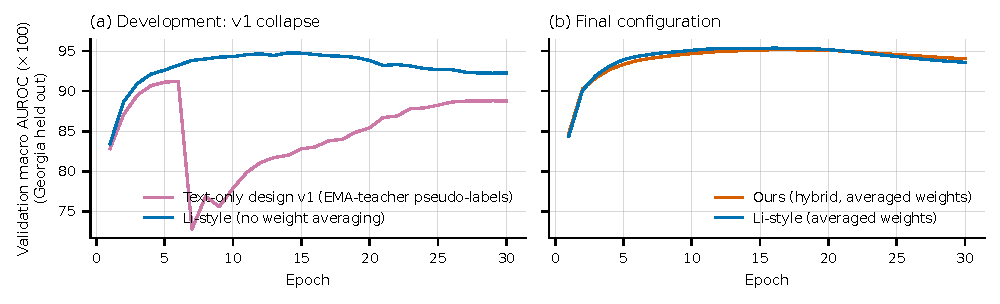
\includegraphics[width=\textwidth]{generated/fig_curves.pdf}
\caption{Validation macro AUROC per epoch with Georgia held out. (a) Design v1 collapses when pseudo-labels take effect (epoch 7), whereas the Li-style baseline trained identically without pseudo-labels does not. (b) The final hybrid configuration and the Li-style baseline, both with weight averaging (seed 1), train smoothly and select a checkpoint around epoch 15.}\label{fig:curves}
\end{figure}

\paragraph{Diagnosis of the collapse.}
Inspection of the logged pseudo-label statistics identified three interacting causes. (i) Hard pseudo-labels were biased towards positives on diagnoses whose implication parent is completed: implication completion (Eq.~\eqref{eq:rules}) creates parent columns that are observed only when positive, so the model learns high parent probabilities, and the teacher then turns unobserved parent entries into confident positive pseudo-labels, which feed back into the student. (ii) With a constant momentum of 0.999 and no warm-up, the teacher still contained $0.999^{t}$ of its random initialization after $t$ steps, about 20\% when pseudo-labels began to take effect, so early pseudo-labels came from a partly random network. (iii) Hard thresholds turned small teacher biases into full-weight targets. These causes are specific to pseudo-labeling and implication completion, which is consistent with the ablations in which removing either one improved seen-diagnosis accuracy.

\subsection{Design v2: corrected text-only head}\label{secA2:v2}
The second design kept a single text-anchored head and corrected each cause: soft rather than hard pseudo-targets, applied from the end of the learning-rate warm-up; implication used as a label-free consistency constraint (the probability of a parent should not be lower than that of its child) instead of positive-only completed targets; the momentum warm-up of Eq.~\eqref{eq:ema}; and validation, selection and testing of the averaged weights. Because a pure text head lacks the per-diagnosis capacity of a linear head, a class-specific residual for seen diagnoses was also evaluated: a per-diagnosis bias, a per-diagnosis read-out of the diagnosis' own cross-attended evidence, a per-diagnosis read-out of the pooled tokens, or both read-outs. Unseen diagnoses keep the pure text logit. Table~\ref{tab:sweeps} (top) reports the four candidates and two zero-shot proxies, in which five diagnoses annotated by PTB-XL and Shaoxing--Ningbo were withheld from training and scored on the validation split. The configuration with both read-outs (S1) was selected by the pre-registered rule; with three seeds on all folds it reached 85.66 (Table~\ref{tab:ablation}, ``text head only''), above v1 but still 0.6 points below the masked and Li-style baselines with weight averaging. The collapse was eliminated, but a single text-anchored head, even with a class-specific residual, did not reach the seen-diagnosis accuracy of a linear head.

\begin{table}[!htbp]
\centering\footnotesize
\caption{Configuration sweeps on one fold (Georgia held out, seed 0). Selection used the source validation macro AUROC only; ``zero-shot proxy'' is the validation macro AUROC on five diagnoses withheld from training, at the selected epoch. The reference is Li-style with weight averaging on the same fold (validation 95.31).}\label{tab:sweeps}
\begin{tabular}{llcc}
\toprule
 & Configuration & Validation AUROC & Zero-shot proxy \\
\midrule
\multicolumn{4}{l}{\emph{v2 sweep (text-only head)}} \\
S1 & both residual read-outs, averaged weights & \textbf{94.56} & 68.6 \\
S2 & as S1, student weights & 94.12 & -- \\
S3 & query read-out only, averaged weights & 94.37 & -- \\
S4 & no residual, averaged weights & 93.90 & 67.9 \\
\midrule
\multicolumn{4}{l}{\emph{Hybrid sweep (linear head + text head)}} \\
H1 & linear scoring of seen diagnoses & 95.19 & -- \\
H2 & mean-probability fusion (selected) & \textbf{95.27} & 69.9 \\
H3 & as H2, detached text head & 95.33 & 66.4 \\
H4 & as H2, with soft pseudo-labels & 95.23 & -- \\
\bottomrule
\end{tabular}
\end{table}

\subsection{Design v3: hybrid head}\label{secA2:hybrid}
The final design keeps the linear head of the baselines unchanged and adds the pure text-anchored head on the same encoder, as described in Section~\ref{sec:head}. Four variants were compared (Table~\ref{tab:sweeps}, bottom). The pre-registered rule was: highest validation AUROC, with ties within 0.001 broken in favour of the simpler configuration in the order H1 $<$ H2 $<$ H3 $<$ H4, and the zero-shot proxy of the selected configuration checked against that of the detached variant. H3 had the highest validation AUROC but was within 0.001 of H2, which is simpler (it needs no gradient stopping) and had the higher zero-shot proxy (69.9 against 66.4); H2 was therefore selected. H2 did not exceed the Li-style reference on validation (95.27 against 95.31). For this case the rule contained a fallback: H1 was to be chosen if its zero-shot proxy passed a guard (at least 65.9, i.e.\ 2 points below the pure text head of v2) and its validation AUROC was within 0.002 of the reference, so that the claim would rest on the seen-diagnosis performance of the linear head plus the zero-shot ability of the text head. H1 met both conditions (95.19, proxy 69.9). \emph{We did not apply this fallback} and kept H2 as the main configuration; we report the deviation here. Both configurations were subsequently run on all folds with three seeds, H1 as ablation (i) of Table~\ref{tab:ablation}, so the reader can evaluate either choice: H1 has a mean seen-diagnosis AUROC of 86.06 (0.21 below Li-style) and the same unseen-diagnosis AUROC as H2 (67.3 against 67.0), and H2 has 86.57. Had H1 been reported as the main method, the conclusions on unseen diagnoses would be unchanged, and the seen-diagnosis conclusion would be that the method is slightly below, rather than level with, the strongest baselines.

\subsection{Effect of weight averaging}\label{secA2:ema}
Validating, selecting and testing the averaged weights (Eq.~\eqref{eq:ema}) is a generic change that any method can use. Fig.~\ref{fig:ema} compares each baseline with and without it (seed 0, mean over the four held-out databases). It improved every baseline, by 0.33 (DANN) to 1.79 points (naive pooling), and narrowed the spread between baselines. All comparisons in the main text therefore use weight averaging for every method; without it, the baselines would have been 0.3--1.8 points weaker and the advantage of the proposed method correspondingly overstated.

\begin{figure}[!htbp]
\centering
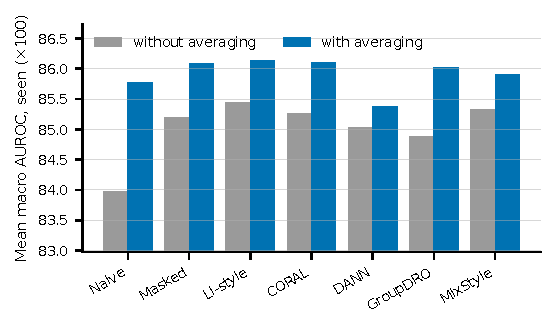
\includegraphics[width=0.62\textwidth]{generated/fig_ema.pdf}
\caption{Seen-diagnosis macro AUROC of each baseline with and without weight averaging (seed 0, mean over four held-out databases).}\label{fig:ema}
\end{figure}

\end{appendices}

\bibliography{references}

\end{document}
